\chapter{Specific Requirements}
\label{chap:specific-requirements}

\par This chapter describes the specific requirements of the Best Bike Paths (BBP) system. It provides detailed information on the external interfaces through which users and external services interact with the system. These requirements supplement the functional and domain descriptions by clarifying how BBP is accessed, which devices it relies on, and how it communicates with external data sources.

\section{External Interface Requirements}
\label{sec:external-interface-requirements}

\subsection{User Interfaces}
\label{subsec:user-interfaces}

\par The primary user interface of BBP is designed with a mobile-first approach, as cyclists typically interact with the system through smartphones while biking or during breaks. The interface allows registered users to access core functionalities, including:

\begin{itemize}
    \item starting, pausing, and stopping the recording of a trip to track cycling activities;
    \item visualizing the reconstructed path, associated statistics (e.g., speed, distance), and enriched meteorological information;
    \item submitting manual data regarding path status and obstacles;
    \item confirming or correcting automatically detected information (e.g., potholes) to prevent false positives before publication;
    \item browsing existing bike paths between a specific origin and destination, visualized based on their calculated score;
    \item accessing previously recorded trips and personal contributions.
\end{itemize}

\par The user interface focuses on clarity and ease of interaction. While a web interface may be provided for browsing statistics on larger screens, the automated data acquisition features rely on a mobile application environment.

\subsection{Hardware Interfaces}
\label{subsec:hardware-interfaces}

\par BBP relies heavily on smartphones, which act as the primary sensing and interaction devices. The system requires access to the following hardware components:

\begin{itemize}
    \item \textbf{GPS and location sensors} to reconstruct the followed path and determine speed (used to infer biking activity);
    \item \textbf{Accelerometers and gyroscopes} to detect significant device movements and vibrations that suggest the presence of potholes or other obstacles;
    \item \textbf{Networking hardware} (Wi-Fi or mobile data) to allow synchronization of data and retrieval of external information;
    \item \textbf{Local device storage} to buffer trip data before upload.
\end{itemize}

\subsection{Software Interfaces}
\label{subsec:software-interfaces}

\par BBP interacts with several external software services and platform-level interfaces necessary to provide complete and accurate information. These include:

\begin{itemize}
    \item \textbf{Map service interfaces}, which provide geographic data and visualization capabilities for the paths;
    \item \textbf{Weather information providers}, which allow the system to enrich trip data with meteorological information (weather conditions, temperature, wind speed);
    \item \textbf{Mobile operating system APIs}, which grant access to device sensors such as GPS, accelerometers, and gyroscopes.
\end{itemize}

\par These external services are accessed programmatically by the BBP system. Specific technical details regarding protocols and data formats are deferred to the Design Document (DD).

\subsection{Communication Interfaces}
\label{subsec:communication-interfaces}

\par Communication between BBP components and external services relies on secure and widely adopted web protocols. Specifically:

\begin{itemize}
    \item \textbf{HTTPS} is used for all communication between the client application and the backend server to ensure data security.
    \item \textbf{RESTful service endpoints} are used for structured data exchange between clients and the backend.
    \item \textbf{External API calls} are used to retrieve data from map and weather services.
\end{itemize}

\par No additional legacy communication channels are required by the system specification.

\section{Functional Requirements}
\label{sec:functional-requirements}

\subsection{Requirements List}
\label{subsec:requirements-list}

\newcounter{requirementCounter}
\setcounter{requirementCounter}{0}
\newcommand{\nextRequirementID}{
    \stepcounter{requirementCounter}R\ifnum\value{requirementCounter}<10 0\fi\arabic{requirementCounter}
}

\begin{longtable}{|l|p{0.9\textwidth}|}
\hline
\textbf{ID} & \textbf{Requirement} \\
\hline \hline

% -----------------------------------
% USER AUTH / ACCOUNT
% -----------------------------------
\nextRequirementID &
The system shall allow cyclists to create a registered account using a valid email address. \\
\hline

\nextRequirementID &
The system shall allow registered cyclists to log in and log out securely. \\
\hline

\nextRequirementID &
The system shall allow unregistered cyclists to access publicly available information without authentication. \\
\hline

% -----------------------------------
% TRIP RECORDING
% -----------------------------------
\nextRequirementID &
The system shall allow registered cyclists to start a new trip recording session. \\
\hline

\nextRequirementID &
The system shall record geographic coordinates at regular intervals during a trip. \\
\hline

\nextRequirementID &
The system shall generate a sequence of \texttt{TrackPoint} objects for every recorded trip. \\
\hline

\nextRequirementID &
The system shall compute summary statistics for each trip, including distance, duration, and average speed. \\
\hline

\nextRequirementID &
The system shall allow cyclists to set the acquisition mode (manual or automatic) for a trip. \\
\hline

\nextRequirementID &
The system shall associate weather conditions with a trip when external weather information is available. \\
\hline

% -----------------------------------
% MANUAL MODE
% -----------------------------------
\nextRequirementID &
The system shall allow cyclists using manual acquisition mode to manually specify the streets forming their trip path. \\
\hline

% -----------------------------------
% OBSTACLE REPORTS
% -----------------------------------
\nextRequirementID &
The system shall allow registered cyclists to submit obstacle reports during or after a trip. \\
\hline

\nextRequirementID &
The system shall mark a newly submitted obstacle report as \texttt{PENDING}. \\
\hline

\nextRequirementID &
The system shall allow cyclists to confirm or reject automatically detected obstacle reports. \\
\hline

\nextRequirementID &
The system shall update the status of an obstacle report to \texttt{CONFIRMED} or \texttt{REJECTED} after user validation. \\
\hline

\nextRequirementID &
The system shall associate confirmed obstacle reports with an existing obstacle or create a new \texttt{Obstacle}. \\
\hline

\nextRequirementID &
The system shall allow cyclists to choose whether an obstacle report is publishable. \\
\hline

% -----------------------------------
% OBSTACLES
% -----------------------------------
\nextRequirementID &
The system shall store each obstacle together with its description and geographic coordinates. \\
\hline

\nextRequirementID &
The system shall associate obstacles with the street on which they are located. \\
\hline

\nextRequirementID &
The system shall update the visibility of an obstacle depending on the cyclist’s publishability settings. \\
\hline

% -----------------------------------
% PATH INFORMATION
% -----------------------------------
\nextRequirementID &
The system shall represent bike paths as sequences of streets between an origin and a destination. \\
\hline

\nextRequirementID &
The system shall display the current status and score of each bike path. \\
\hline

\nextRequirementID &
The system shall allow registered cyclists to submit \texttt{PathStatusReport} entries for any bike path. \\
\hline

\nextRequirementID &
The system shall allow cyclists to specify whether their path status report is publishable. \\
\hline

\nextRequirementID &
The system shall update the aggregated status or score of a bike path based on submitted path status reports. \\
\hline

% -----------------------------------
% BROWSING DATA
% -----------------------------------
\nextRequirementID &
The system shall allow cyclists to browse all publicly available bike paths. \\
\hline

\nextRequirementID &
The system shall display the current condition of streets, including reported obstacles. \\
\hline

\nextRequirementID &
The system shall allow cyclists to browse their previously recorded trips. \\
\hline

\nextRequirementID &
The system shall allow cyclists to view details of each trip, including weather, track points, and obstacle reports. \\
\hline

% -----------------------------------
% DATA PUBLISHABILITY / PRIVACY
% -----------------------------------
\nextRequirementID &
The system shall allow cyclists to mark any trip-related data (e.g., obstacle reports, path status reports) as publishable or private. \\
\hline

\nextRequirementID &
The system shall ensure that private reports are not shown to other users. \\
\hline

% -----------------------------------
% EXTERNAL DATA INTEGRATION
% -----------------------------------
\nextRequirementID &
The system shall retrieve weather data from an external weather provider when available. \\
\hline

\nextRequirementID &
The system shall retrieve map and geographic information from an external map provider. \\
\hline

% -----------------------------------
% ERROR HANDLING / VALIDATION
% -----------------------------------
\nextRequirementID &
The system shall notify the user when sensors required for automatic acquisition mode are unavailable. \\
\hline

\nextRequirementID &
The system shall notify the user if GPS signal quality is insufficient to record a trip. \\
\hline

\nextRequirementID &
The system shall prevent the submission of incomplete or invalid obstacle reports. \\
\hline

\caption{System Requirements Table}
\label{tab:requirements-table}
\end{longtable}


\subsection{Use Case Diagrams}
\label{subsec:use-case-diagrams}

\begin{figure}[H]
    \centering
    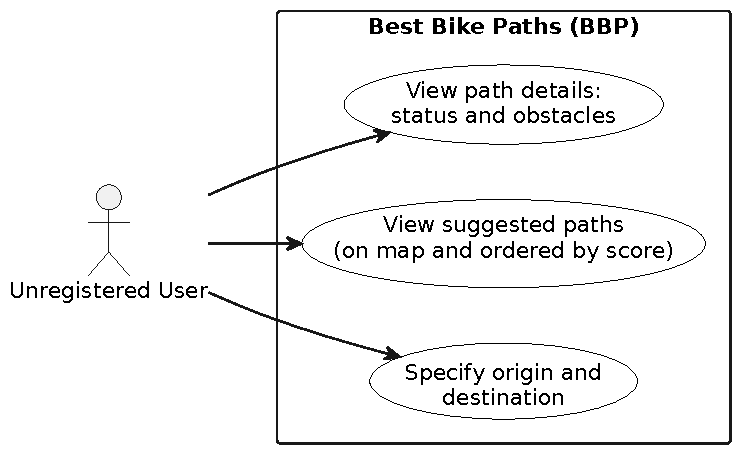
\includegraphics[width=0.9\textwidth]{Images/UC/UC_Unregistered_User.pdf}
    \caption{Unregistered User abilities - Use Case Diagram}
    \label{fig:use-case-diagram-unregistered-user}
\end{figure}

\begin{figure}[H]
    \centering
    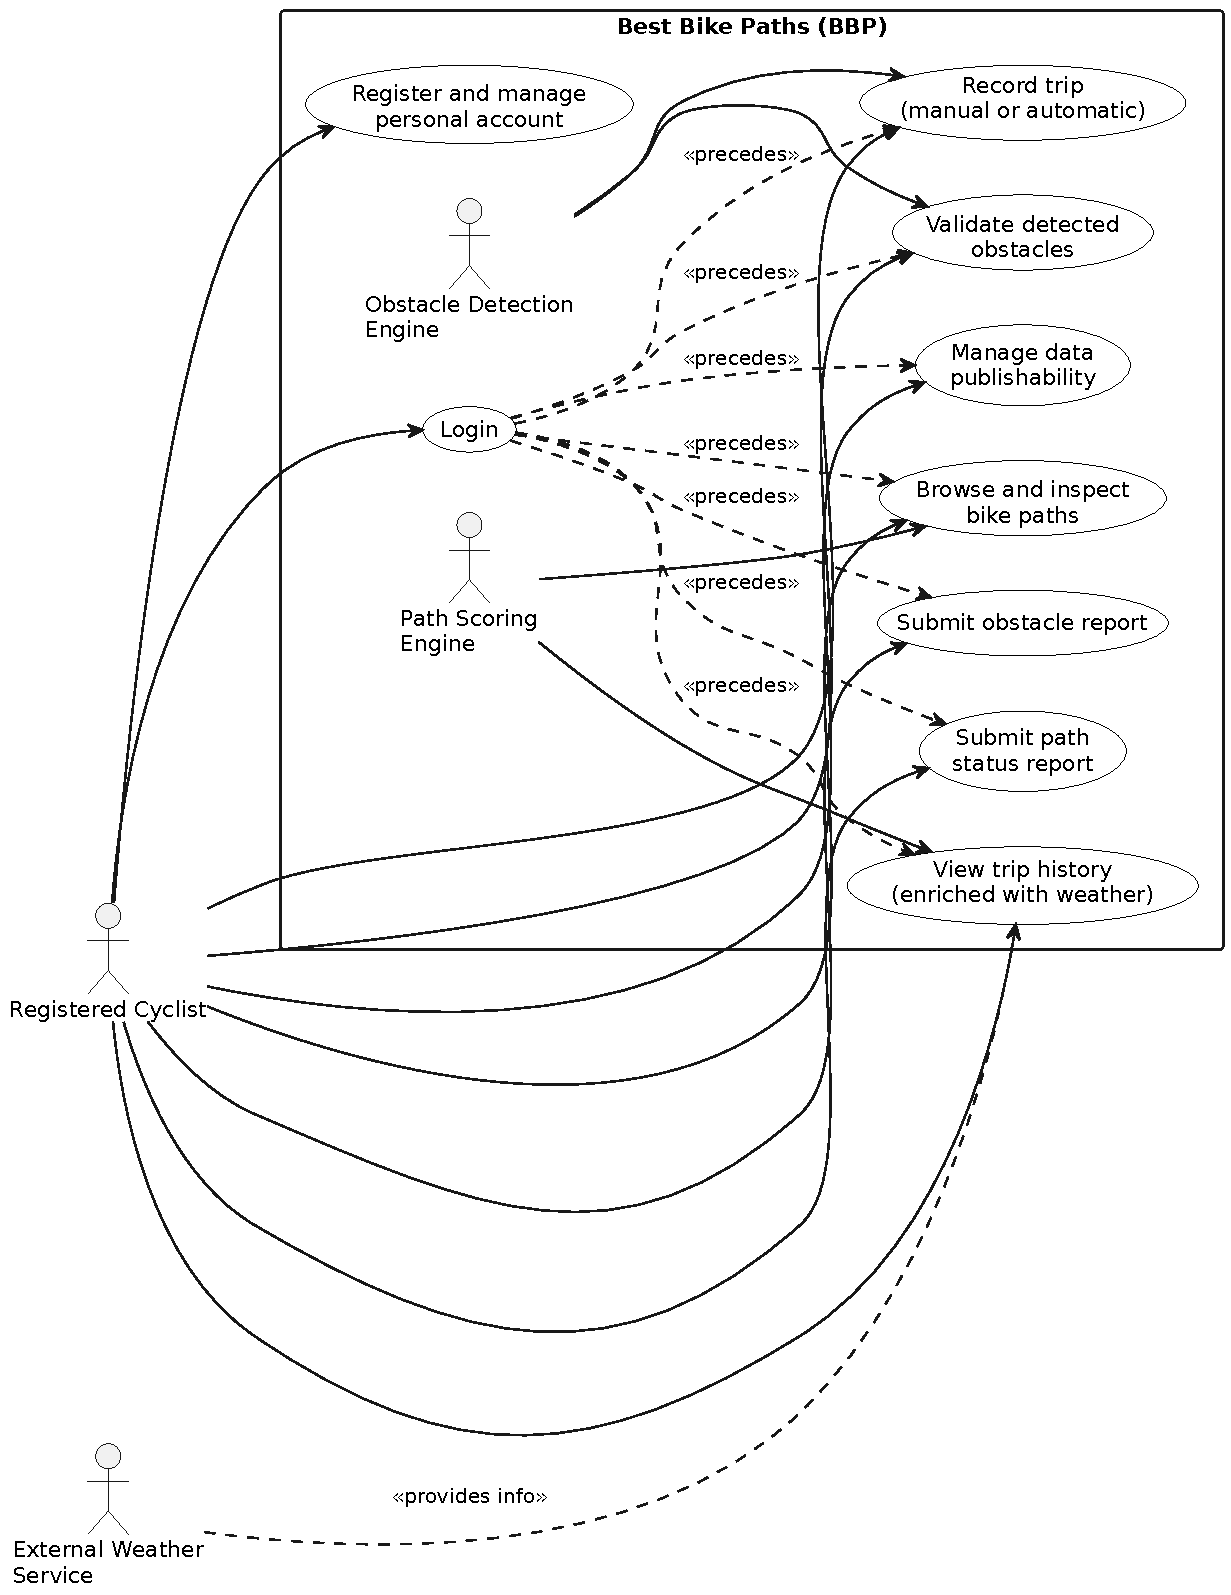
\includegraphics[width=0.9\textwidth]{Images/UC/UC_Registered_Cyclist.pdf}
    \caption{Registered Cyclist abilities - Use Case Diagram}
    \label{fig:use-case-diagram-registered-cyclist}
\end{figure}

\begin{figure}[H]
    \centering
    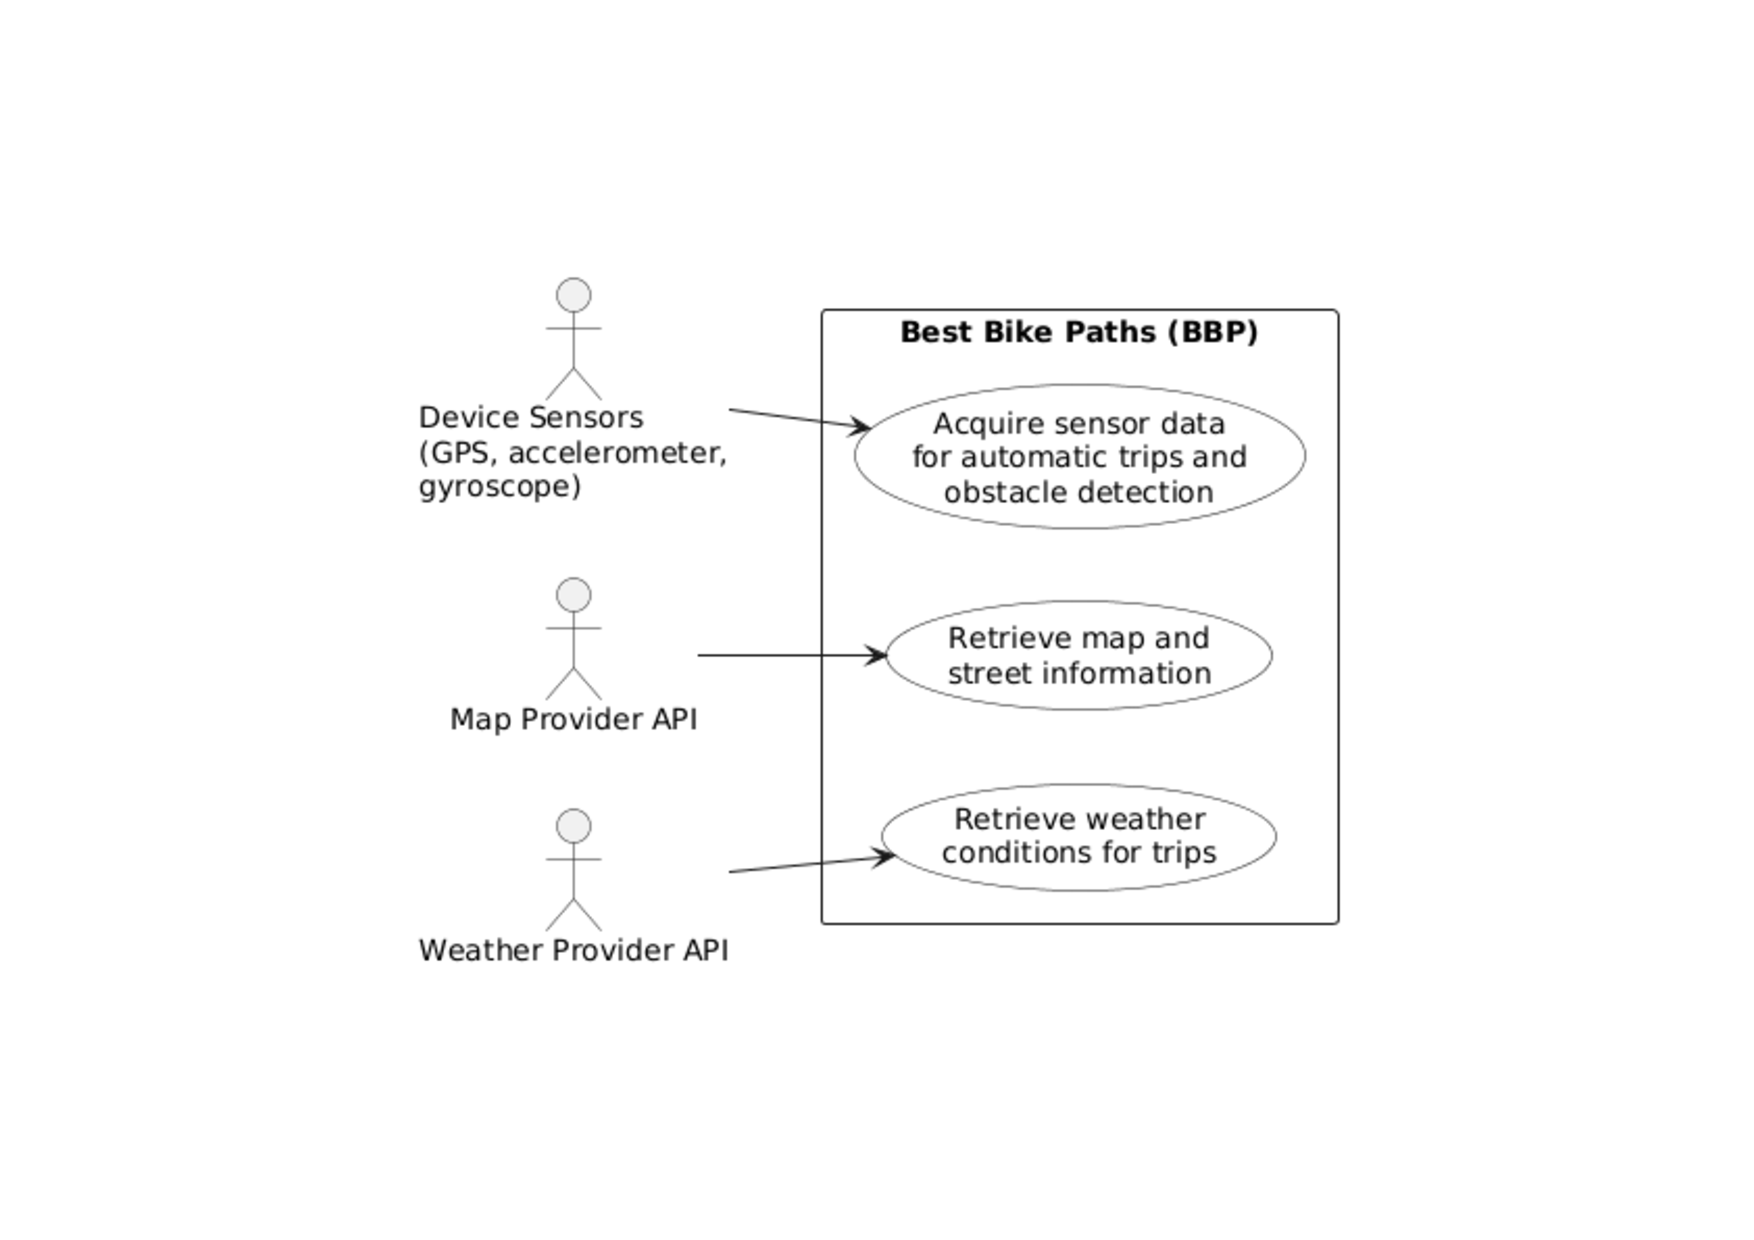
\includegraphics[width=0.9\textwidth]{Images/UC/UC_System_Actors.pdf}
    \caption{System and external services - Use Case Diagram}
    \label{fig:use-case-diagram-system-actors}
\end{figure}

\subsection{Use Cases}
\label{subsec:use-cases}

\par In this section, a detailed description of the main use cases of the system is presented.
Each use case is described by actors, entry conditions, flow of events, exit conditions, and exceptions.
The use case diagram shows the messages exchanged between the actors and the system and the functions called by them.

% 01
\subsubsection{UC00: Cyclist registration}
\label{subsubsec:cyclist-registration}

\begin{center}
\begin{longtable}{|l|p{0.75\linewidth}|}
    \hline
    \textbf{Actors:}           
    & Cyclist (unregistered user)                                                                 \\
    \hline

    \textbf{Entry Conditions:} 
    & \begin{itemize}
          \item The cyclist has access to the BBP application or web interface.
          \item The cyclist has a valid email address.
       \end{itemize}                                                                              \\
    \hline

    \textbf{Flow of Events:}   
    & \begin{enumerate}
          \item The cyclist opens the BBP application or web interface.
          \item The cyclist selects the option \emph{Register} or \emph{Create account}.
          \item BBP displays the registration form requesting at least email, username, and password.
          \item The cyclist fills in the required fields and submits the form.
          \item BBP forwards the registration data to the backend for validation.
          \item The backend verifies:
                \begin{itemize}
                    \item that the email is not already associated with an existing account,
                    \item that all mandatory fields are present and valid (e.g., email format, password constraints).
                \end{itemize}
          \item If the data are valid and the email is not already registered, the backend creates a new \texttt{RegisteredUser} associated with the provided information.
          \item The backend returns a success response to BBP.
          \item BBP displays a confirmation message and may optionally redirect the cyclist to the login page.
       \end{enumerate}                                                                          \\
    \hline

    \textbf{Exit condition:}   
    & A new \texttt{RegisteredUser} account exists in the system and can be used to log in to BBP. \\
    \hline

    \textbf{Exceptions:}       
    & \begin{enumerate}
          \item The email is already registered: BBP informs the cyclist and suggests logging in or recovering the password.
          \item One or more mandatory fields are missing or invalid: BBP highlights the errors and asks the cyclist to correct them.
          \item The backend is temporarily unavailable or returns an error: BBP shows a generic error message and no account is created.
       \end{enumerate}                                                                          \\
    \hline
\end{longtable}
\end{center}

\begin{figure}[H]
    \centering
    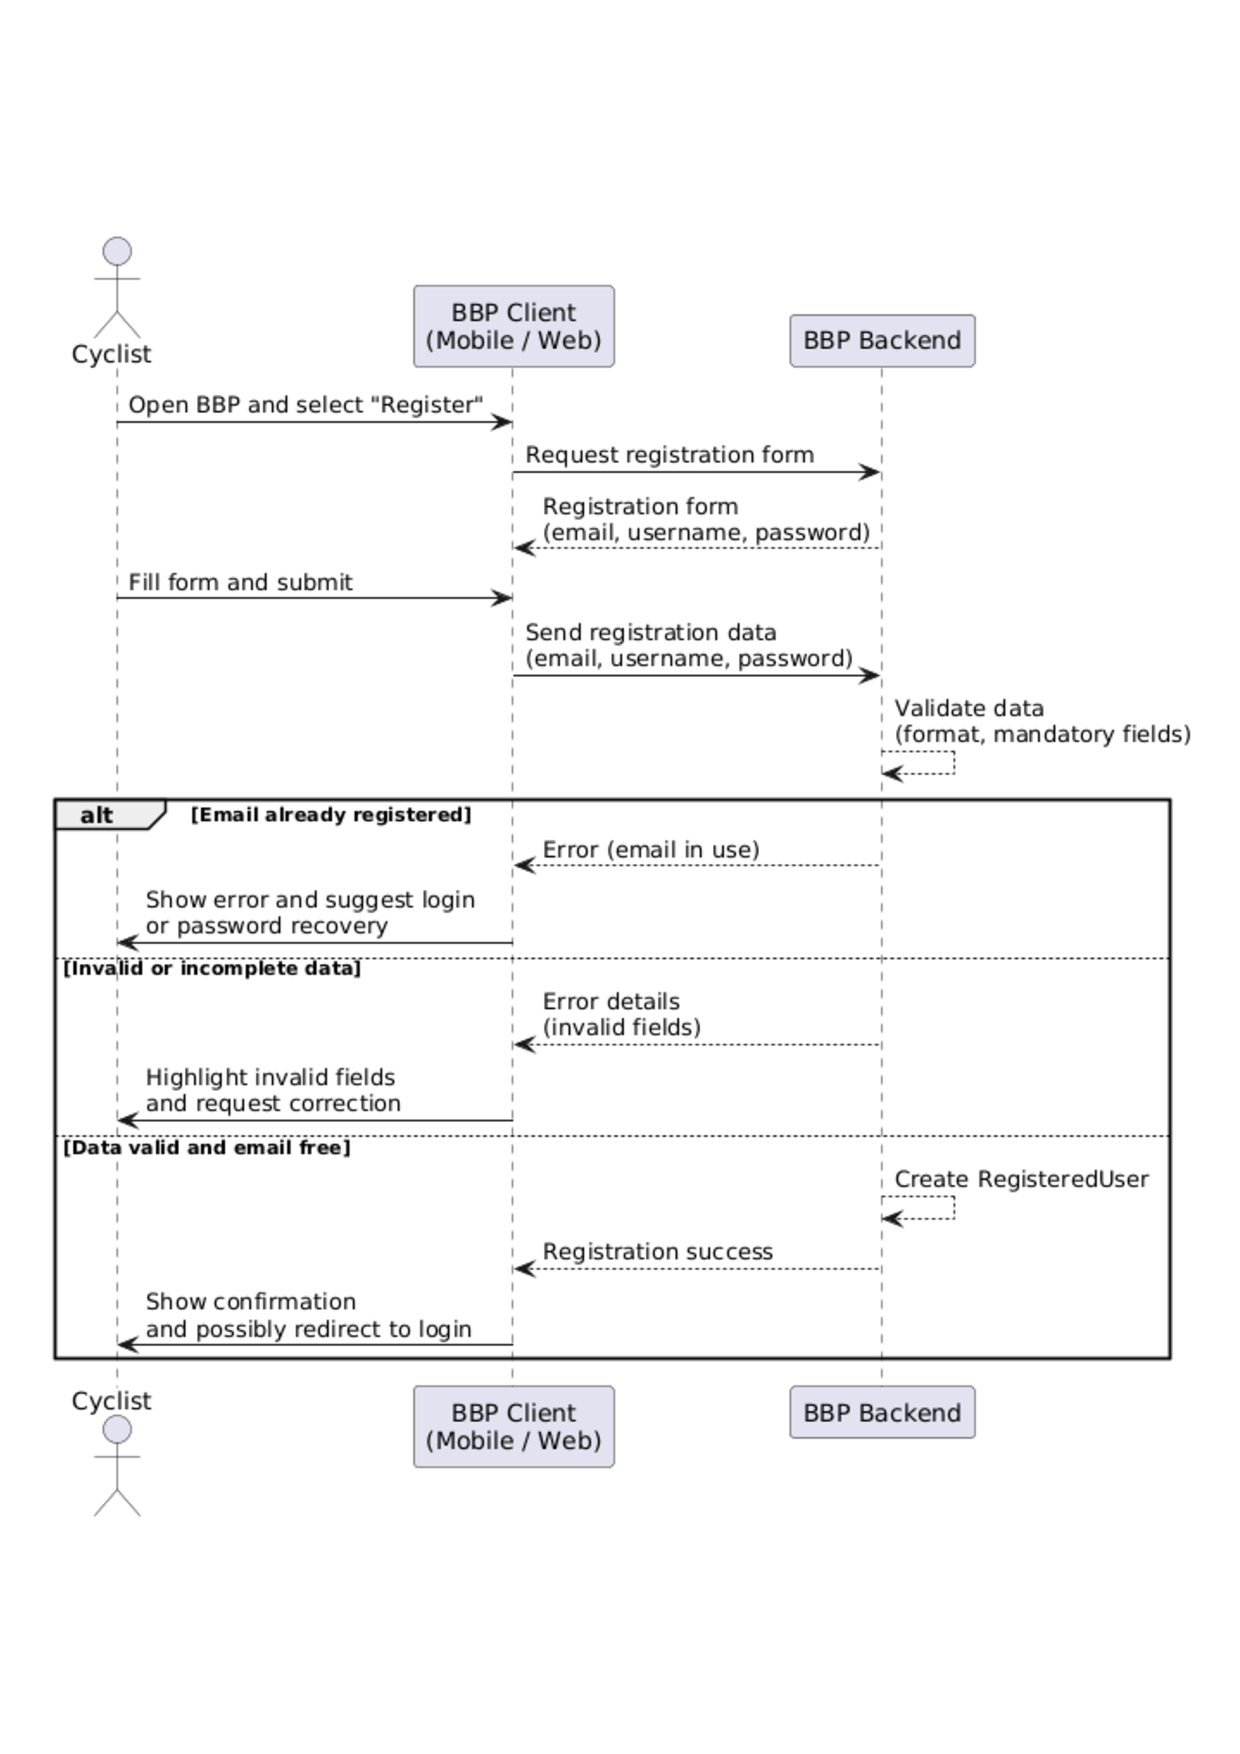
\includegraphics[width=1.0\textwidth]{Images/UC/UC_0.pdf}
    \caption{Cyclist registration - Sequence Diagram}
    \label{fig:use-case-diagram-uc00}
\end{figure}

\subsubsection{UC01: Cyclist login}
\label{subsubsec:cyclist-login}
\begin{center}
    \begin{longtable}{|l|p{0.75\linewidth}|}
        \hline
        \textbf{Actors:}           & Cyclist (registered user)                                                      \\
        \hline
        \textbf{Entry Conditions:} & \begin{itemize}
                                        \item The cyclist has already created a BBP account.
                                        \item The BBP application or web interface is reachable.
                                    \end{itemize}                                                                    \\
        \hline
        \textbf{Flow of Events:}   & \begin{enumerate}
                                        \item The cyclist opens the BBP application or web interface.
                                        \item The cyclist selects the \emph{Login} option.
                                        \item BBP displays the login form requesting email and password.
                                        \item The cyclist enters email and password and submits the form.
                                        \item BBP receives the credentials and forwards them to the authentication service.
                                        \item The authentication service validates the credentials.
                                        \item If validation succeeds, BBP creates a session for the cyclist.
                                        \item BBP redirects the cyclist to the main dashboard (e.g., trips overview or home screen).
                                     \end{enumerate}                                                                 \\
        \hline
        \textbf{Exit condition:}   & The cyclist is logged in and can access personal trips and contributions.      \\
        \hline
        \textbf{Exceptions:}       & \begin{enumerate}
                                        \item The credentials are wrong: BBP shows an error message and asks the cyclist to retry.
                                        \item The account is blocked or deleted: BBP denies access and informs the cyclist.
                                        \item An internal error occurs in the authentication service: BBP shows a generic error message.
                                     \end{enumerate}                                                                 \\
        \hline
    \end{longtable}
\end{center}

\begin{figure}[H]
    \centering
    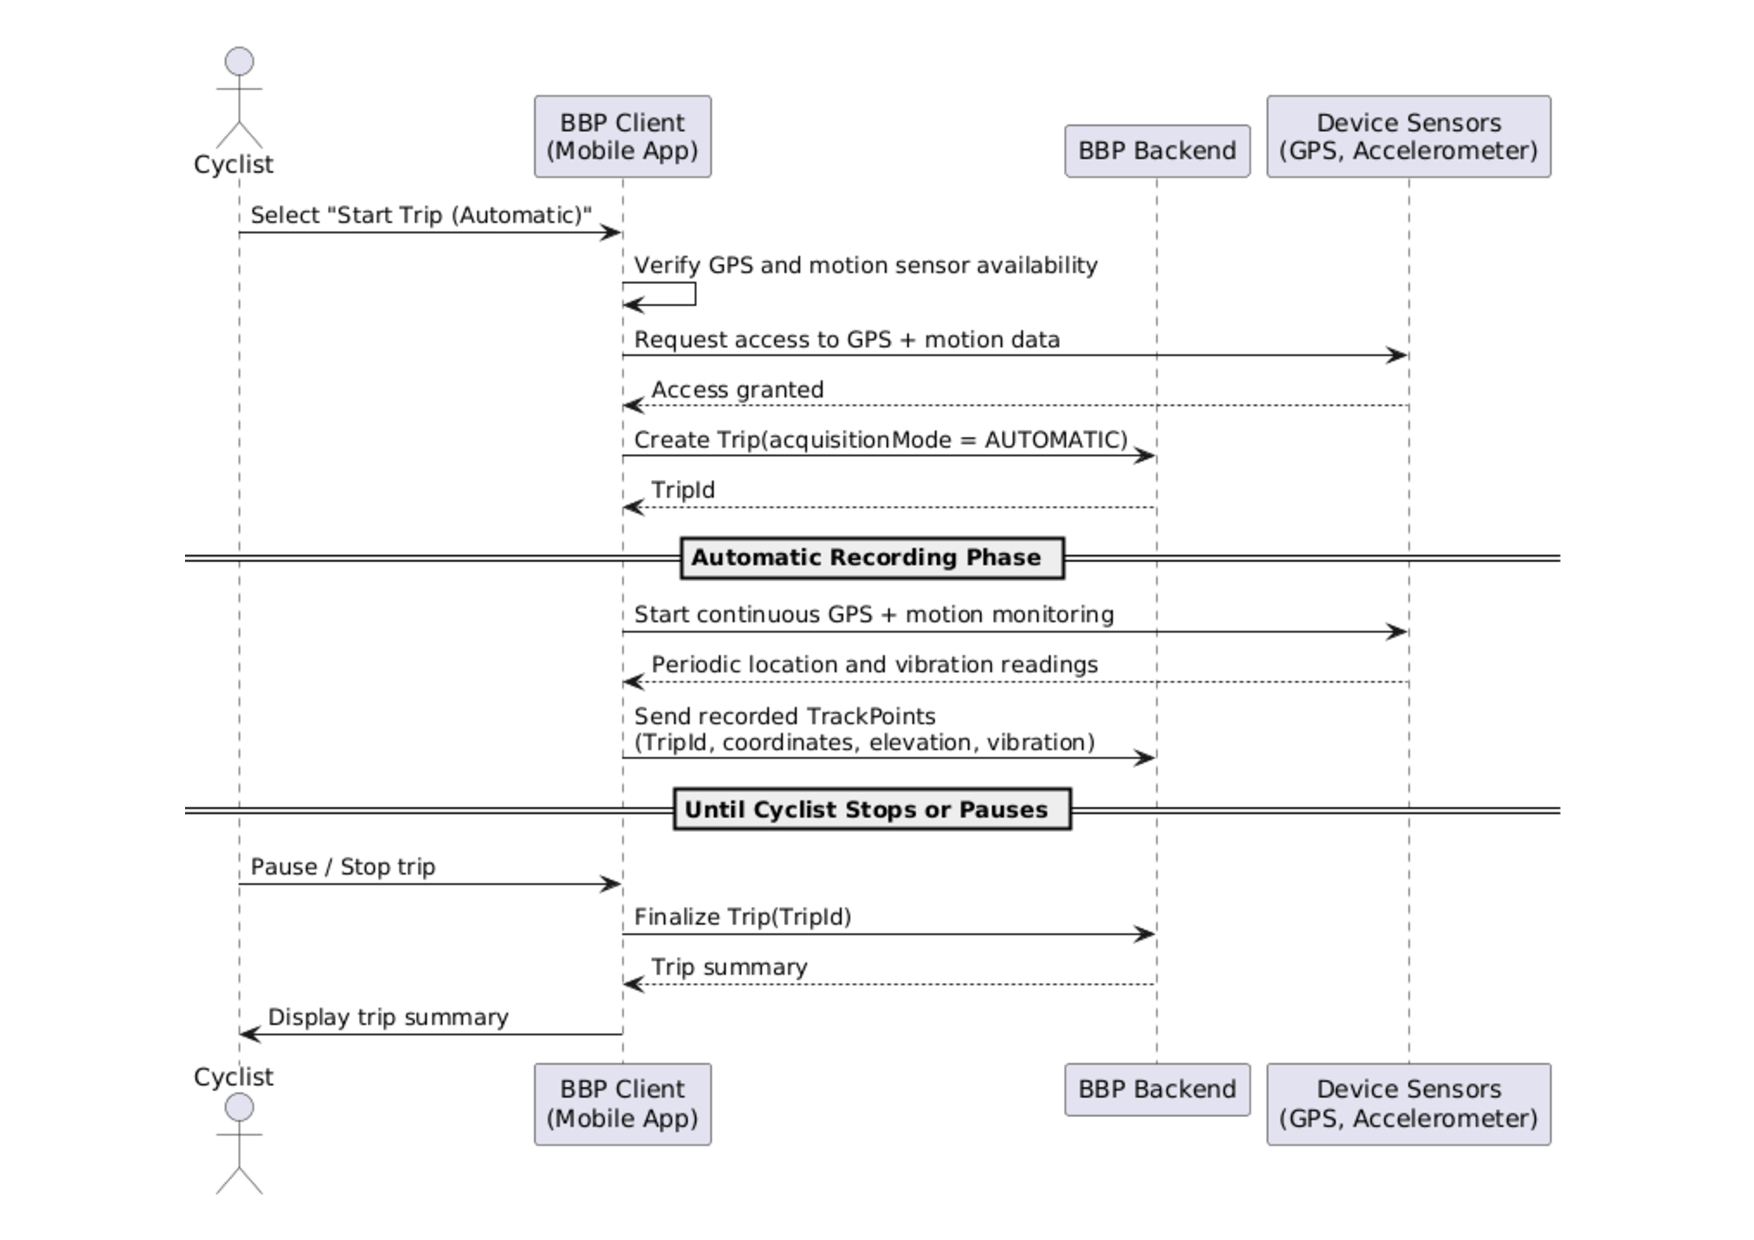
\includegraphics[width=1.0\textwidth]{Images/UC/UC_2.pdf}
    \caption{Cyclist Login - Sequence Diagram}
    \label{fig:use-case-diagram-uc01}
\end{figure}

\subsubsection{UC02: Start automatic trip recording}
\label{subsubsec:start-automatic-trip}

\begin{center}
\begin{longtable}{|l|p{0.75\linewidth}|}
    \hline
    \textbf{Actors:}           
    & Cyclist (registered user)                                                                  \\
    \hline

    \textbf{Entry Conditions:} 
    & \begin{itemize}
          \item The cyclist is authenticated in the BBP system.
          \item The BBP mobile application is installed and running on a device with:
                \begin{itemize}
                    \item GPS and motion sensors (e.g., accelerometer, gyroscope),
                    \item granted permissions for location and motion access.
                \end{itemize}
       \end{itemize}                                                                              \\
    \hline

    \textbf{Flow of Events:}   
    & \begin{enumerate}
          \item The cyclist opens the trip recording section of the application.
          \item The cyclist selects the option \emph{Start Trip (Automatic)}.
          \item BBP verifies that GPS and motion sensors are available and that permissions are granted.
          \item If the checks succeed, BBP sends a request to the backend to create a new \texttt{Trip} with \texttt{acquisitionMode = AUTOMATIC} associated with the cyclist.
          \item The backend creates the Trip and returns the Trip identifier and initial metadata.
          \item BBP starts reading location and motion data from the device sensors at regular intervals.
          \item For each new reading, BBP derives speed and elevation (when available) and sends the data to the backend.
          \item The backend stores each received point as a \texttt{TrackPoint} associated with the Trip.
          \item The trip continues in active automatic recording until the cyclist explicitly stops the recording (handled by a separate use case) or closes the application.
       \end{enumerate}                                                                          \\
    \hline

    \textbf{Exit condition:}   
    & A Trip in automatic acquisition mode is active, and a sequence of \texttt{TrackPoint} objects is being stored for the cyclist. \\
    \hline

    \textbf{Exceptions:}       
    & \begin{enumerate}
          \item GPS or motion sensors are unavailable: BBP informs the cyclist that automatic recording cannot start and suggests enabling sensors or checking the device.
          \item Required permissions are denied: BBP requests the necessary permissions; if the cyclist refuses, the trip is not started.
          \item The backend is temporarily unavailable when creating the Trip: BBP shows an error message and does not start recording.
       \end{enumerate}                                                                          \\
    \hline
\end{longtable}
\end{center}

\begin{figure}[H]
    \centering
    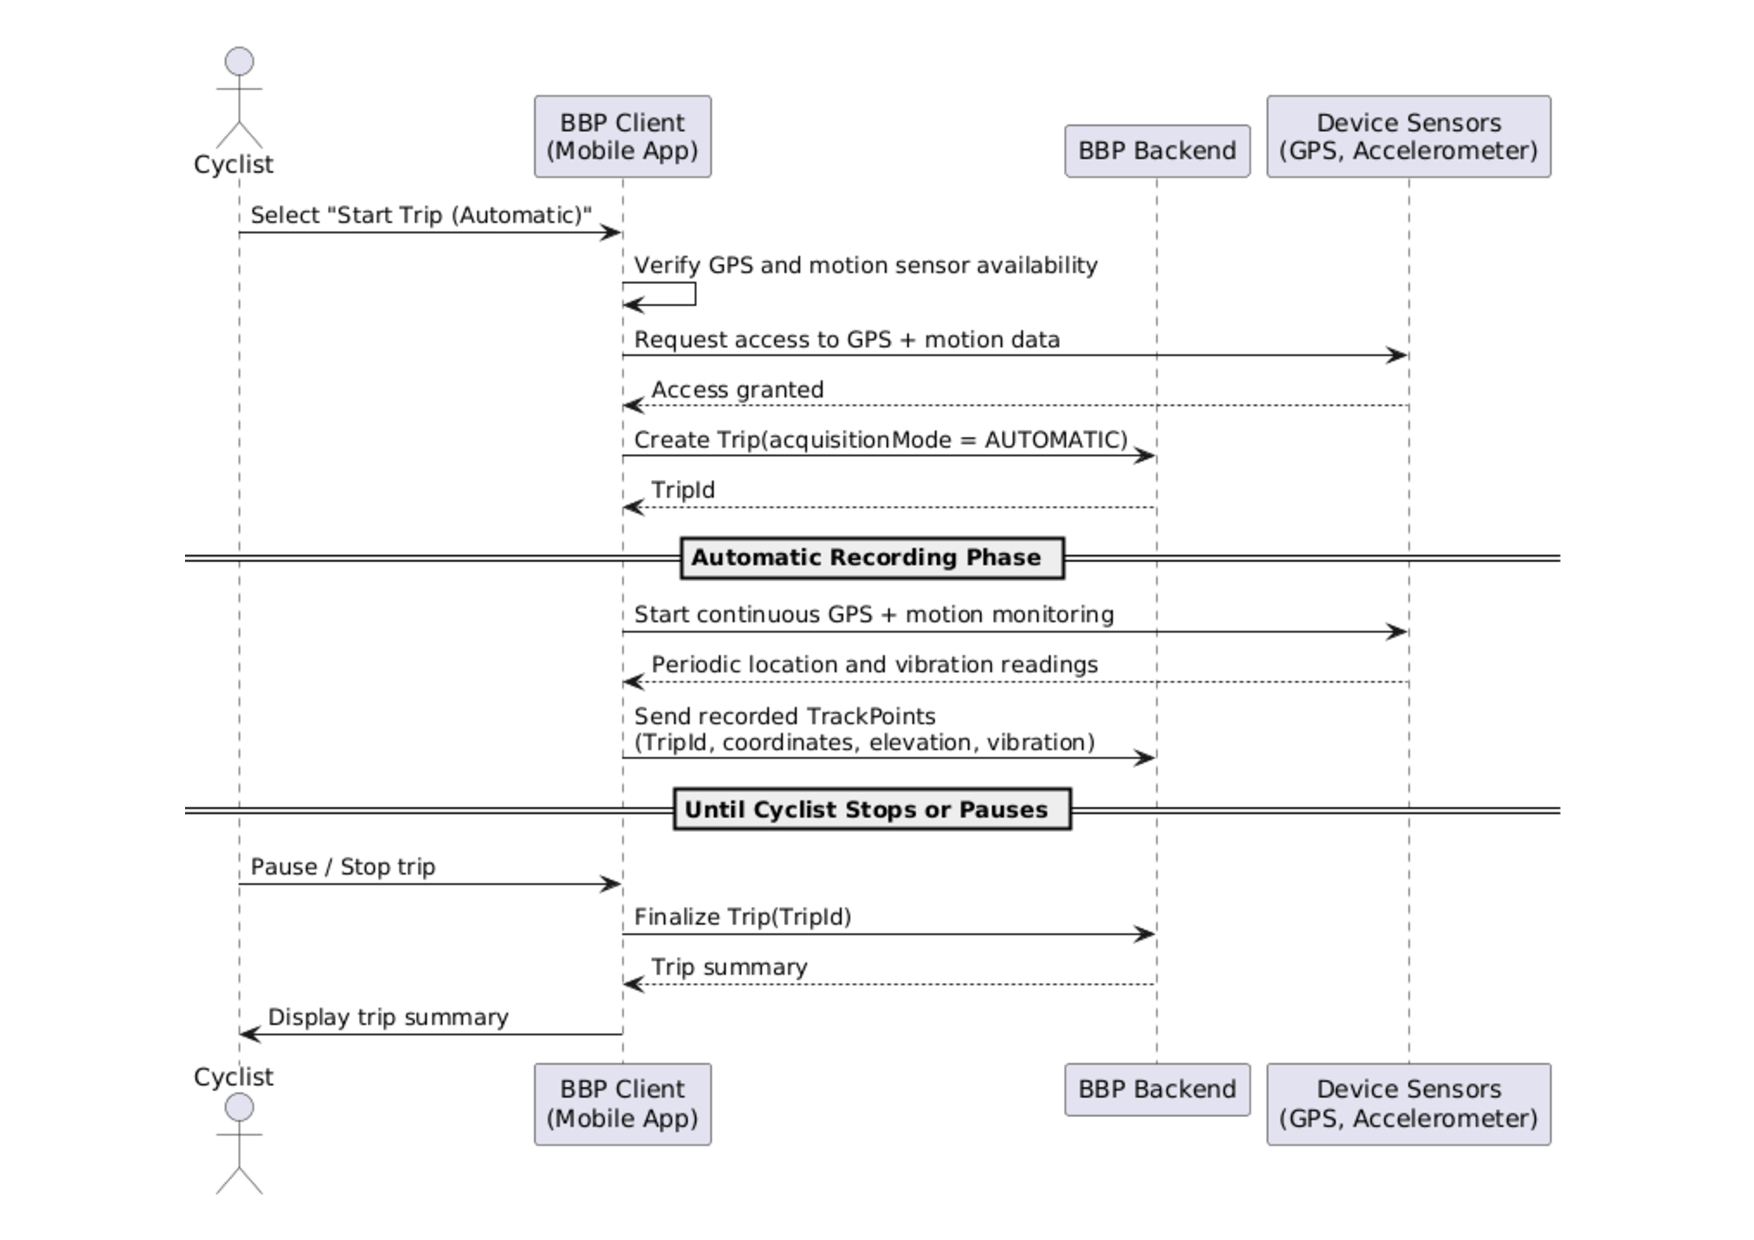
\includegraphics[width=1.0\textwidth]{Images/UC/UC_2.pdf}
    \caption{Start automatic trip recording - Sequence Diagram}
    \label{fig:use-case-diagram-uc02}
\end{figure}


\subsubsection{UC03: Start manual trip recording}
\label{subsubsec:start-manual-trip}

\begin{center}
\begin{longtable}{|l|p{0.75\linewidth}|}
    \hline
    \textbf{Actors:}           
    & Cyclist (registered user)                                                          \\
    \hline

    \textbf{Entry Conditions:} 
    & \begin{itemize}
          \item The cyclist is authenticated in the BBP system.
          \item The BBP application or web interface is reachable.
       \end{itemize}                                                                      \\
    \hline

    \textbf{Flow of Events:}   
    & \begin{enumerate}
          \item The cyclist opens the trip recording section of the application.
          \item The cyclist selects the option \emph{Start Trip (Manual)}.
          \item BBP displays an interface to specify the path manually (for example through a map or street search).
          \item The cyclist selects or enters the streets that will compose the trip path.
          \item BBP validates the selected streets using available map information.
          \item BBP creates a new \texttt{Trip} with \texttt{acquisitionMode = MANUAL} associated with the cyclist.
          \item BBP associates the selected streets with the trip (and with a corresponding \texttt{BikePath}, if applicable).
          \item BBP marks the trip as started and ready to be controlled (pause, resume, stop) by the cyclist.
       \end{enumerate}                                                                    \\
    \hline

    \textbf{Exit condition:}   
    & A Trip in manual acquisition mode is active and associated with a set of streets.  \\
    \hline

    \textbf{Exceptions:}       
    & \begin{enumerate}
          \item One or more street names or selections cannot be validated: BBP notifies the cyclist and requests correction.
          \item The cyclist cancels the manual trip creation before confirming: no Trip is created.
          \item An internal error occurs while creating the Trip: BBP shows an error message and suggests retrying.
       \end{enumerate}                                                                    \\
    \hline
\end{longtable}
\end{center}

\begin{figure}[H]
    \centering
    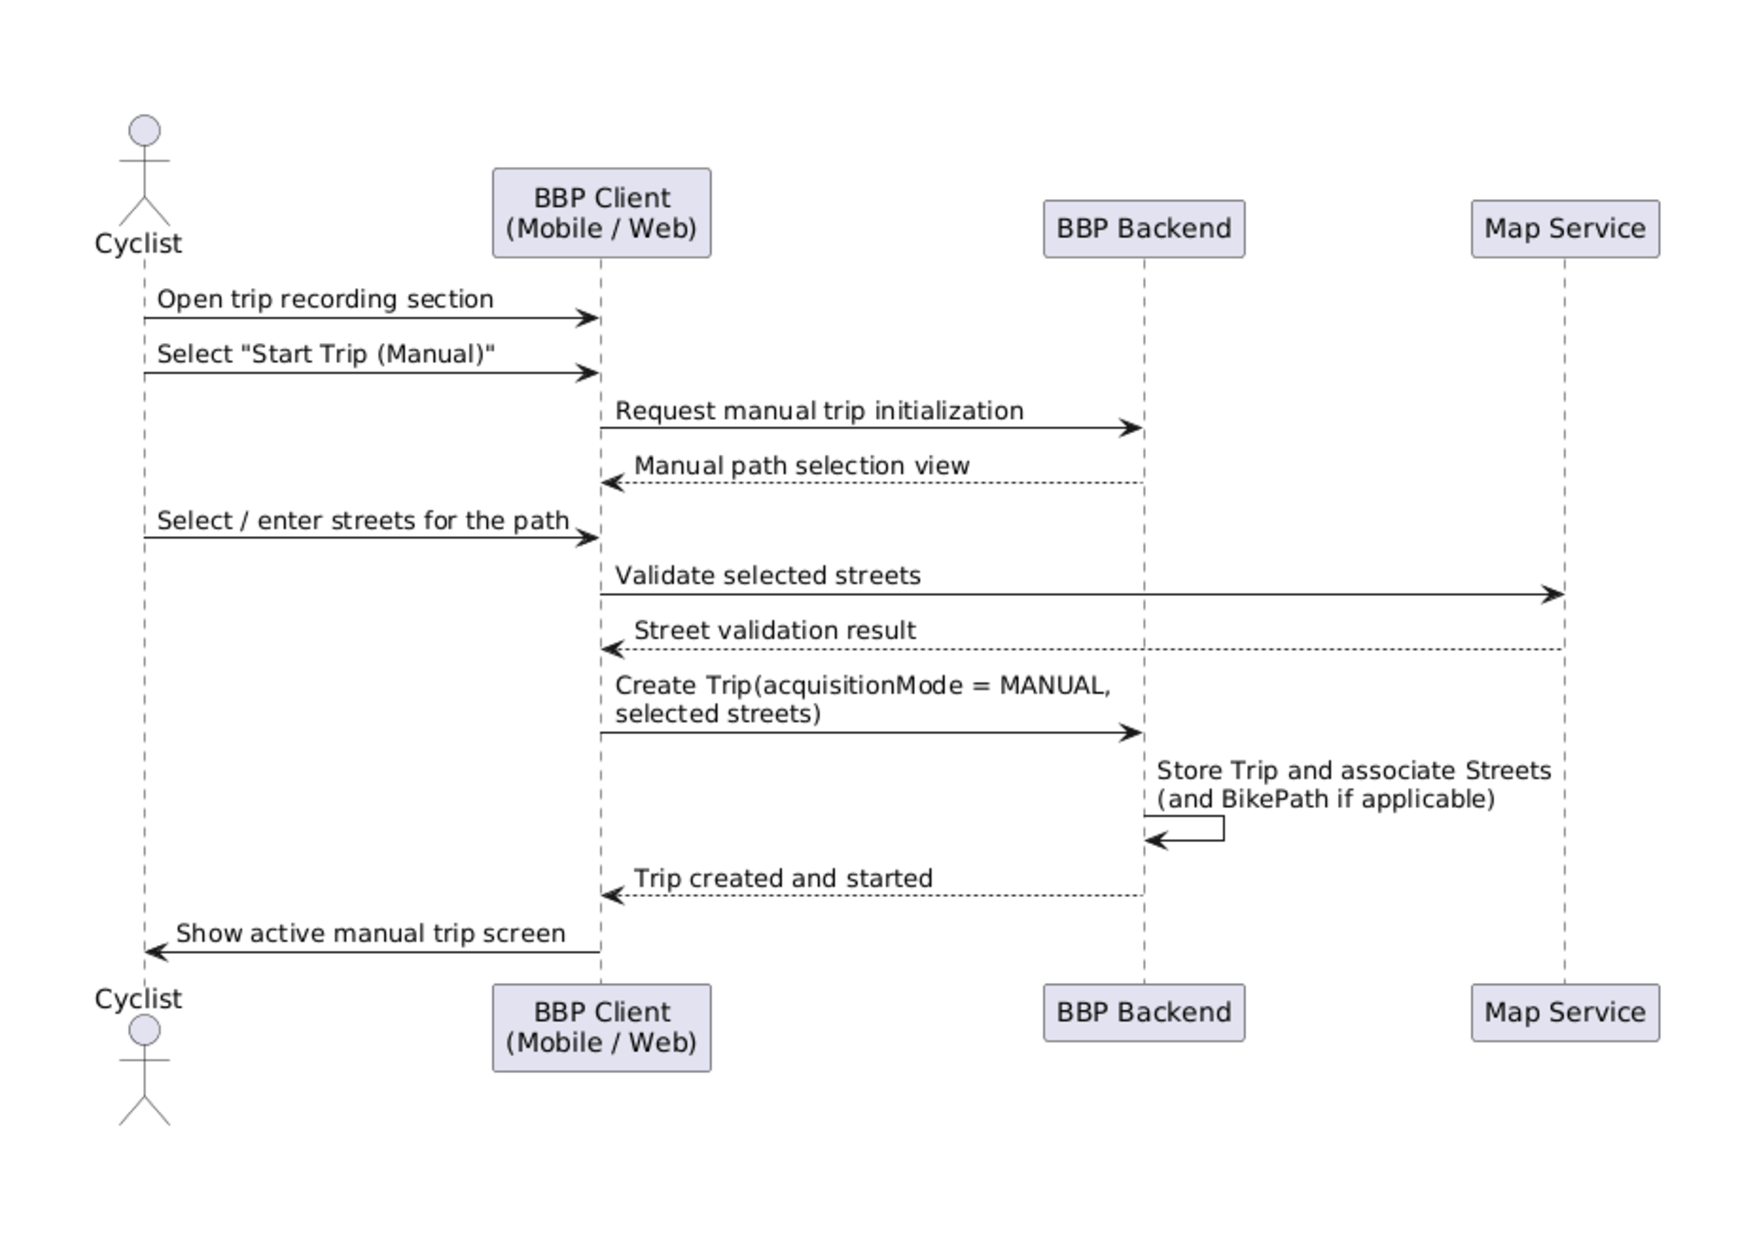
\includegraphics[width=1.0\textwidth]{Images/UC/UC_3.pdf}
    \caption{Start manual trip recording - Sequence Diagram}
    \label{fig:use-case-diagram-uc03}
\end{figure}

\subsubsection{UC04: View trip history and details}
\label{subsubsec:view-trip-history}

\begin{center}
\begin{longtable}{|l|p{0.75\linewidth}|}
    \hline
    \textbf{Actors:}           
    & Cyclist (registered user)                                                               \\
    \hline

    \textbf{Entry Conditions:} 
    & \begin{itemize}
          \item The cyclist is authenticated in the BBP system.
          \item At least one Trip is associated with the cyclist.
       \end{itemize}                                                                           \\
    \hline

    \textbf{Flow of Events:}   
    & \begin{enumerate}
          \item The cyclist navigates to the “My Trips” section of the application.
          \item BBP requests the list of trips associated with the cyclist.
          \item The backend retrieves and sends the list of Trips (with summaries such as date, duration, distance).
          \item The cyclist selects one specific Trip.
          \item BBP requests the detailed information of that Trip.
          \item The backend returns the Trip details including:
                \begin{itemize}
                    \item track points (if automatically acquired),
                    \item associated BikePath (if any),
                    \item weather conditions (if recorded),
                    \item obstacle reports created during the trip.
                \end{itemize}
          \item BBP displays all retrieved information to the cyclist.
       \end{enumerate}                                                                           \\
    \hline

    \textbf{Exit condition:}   
    & The cyclist visualizes the selected Trip with all available details.                      \\
    \hline

    \textbf{Exceptions:}       
    & \begin{enumerate}
          \item No trips exist: BBP displays an empty history message.
          \item Backend temporarily unavailable: BBP displays an error and offers retry.
          \item Trip details incomplete (for example missing map data): BBP displays available parts and warns the user.
       \end{enumerate}                                                                           \\
    \hline
\end{longtable}
\end{center}

\begin{figure}[H]
    \centering
    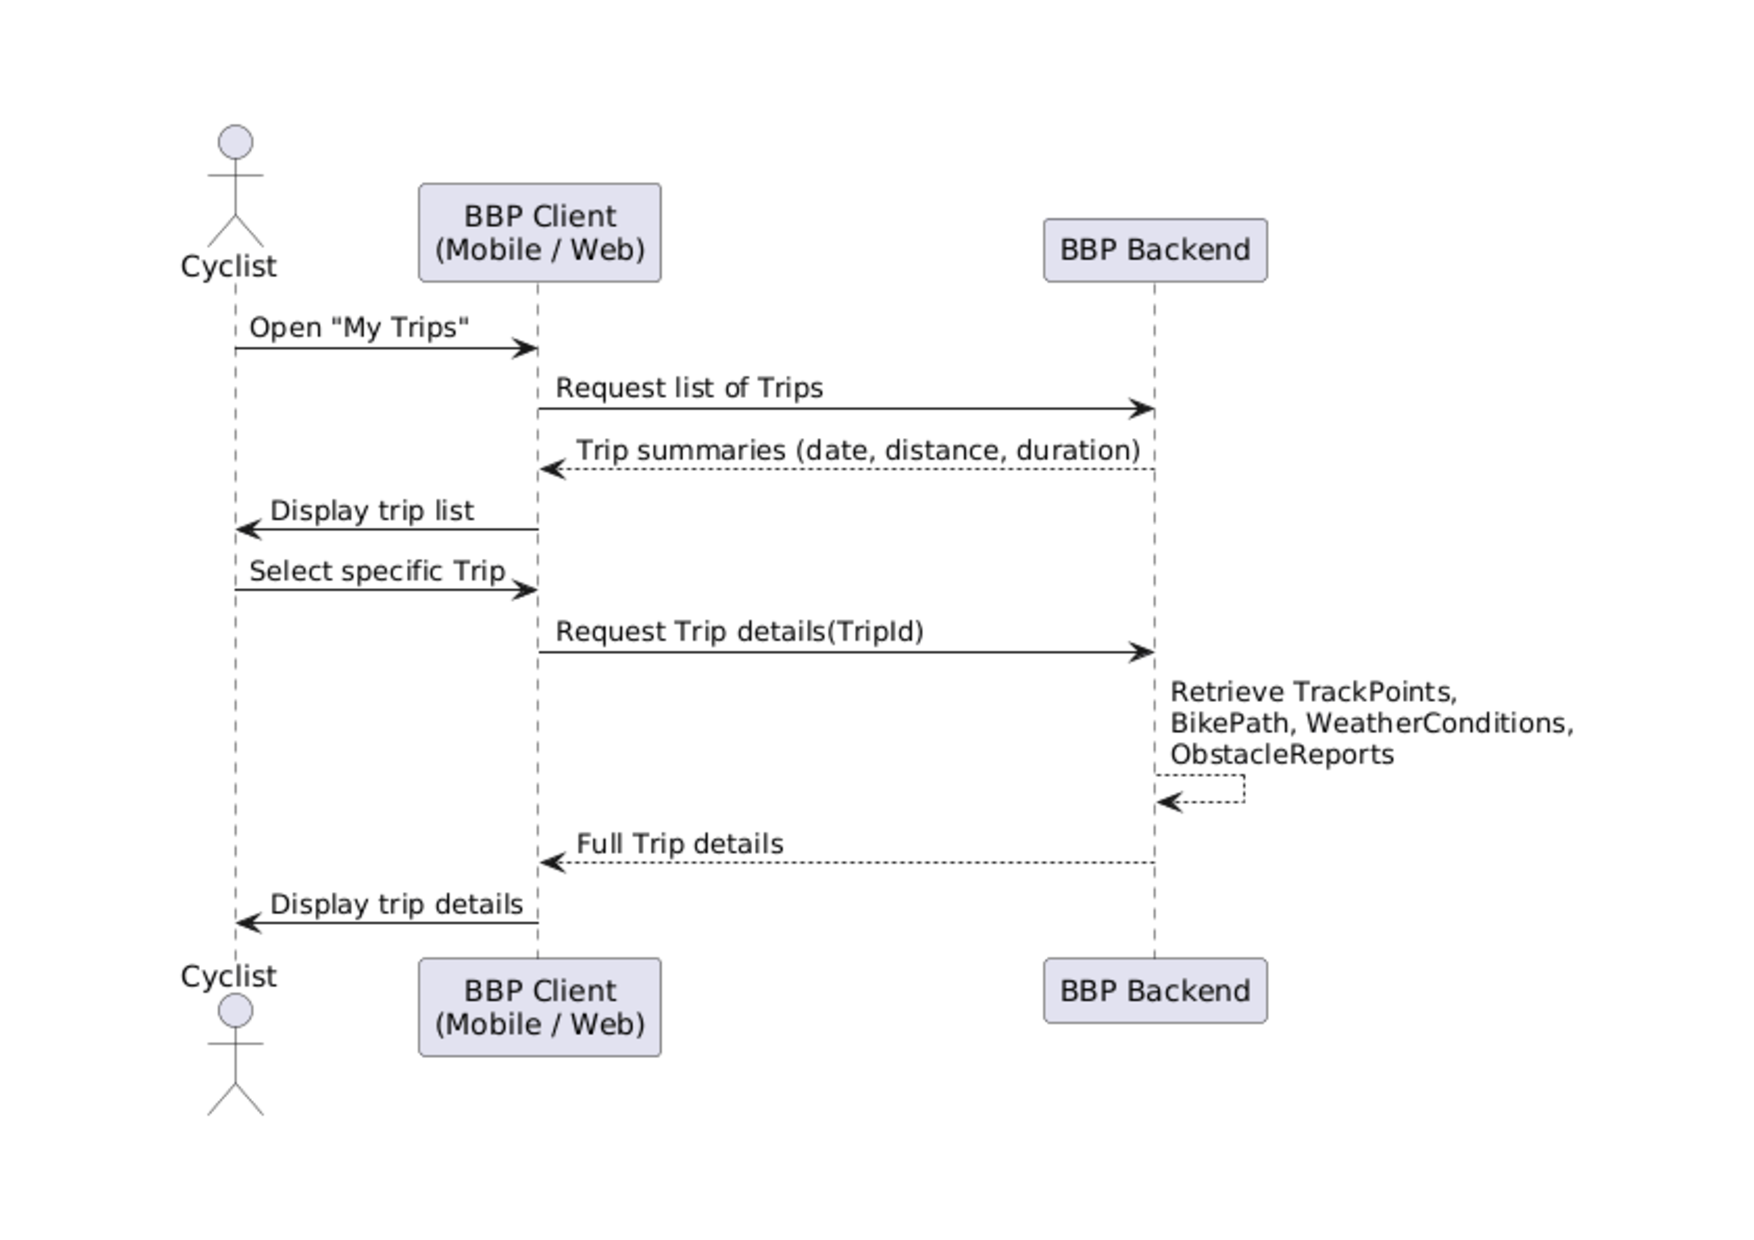
\includegraphics[width=1.0\textwidth]{Images/UC/UC_4.pdf}
    \caption{View trip history and trip details - Sequence Diagram}
    \label{fig:use-case-diagram-uc04}
\end{figure}

% ============================
% UC05: SUBMIT OBSTACLE REPORT
% ============================

\subsubsection{UC05: Submit obstacle report}
\label{subsubsec:submit-obstacle-report}

\begin{center}
\begin{longtable}{|l|p{0.75\linewidth}|}
    \hline
    \textbf{Actors:}           
    & Cyclist (registered user)                                                                      \\
    \hline

    \textbf{Entry Conditions:} 
    & \begin{itemize}
          \item The cyclist is authenticated in the BBP system.
          \item The cyclist has identified a potential obstacle along a street or along a recorded trip.
       \end{itemize}                                                                                 \\
    \hline

    \textbf{Flow of Events:}   
    & \begin{enumerate}
          \item The cyclist selects the \emph{Report obstacle} option from the application.
          \item BBP displays a form requesting the obstacle location (for example map position or current GPS position), a short description, and optional additional notes.
          \item The cyclist provides the mandatory information and optionally adds extra details.
          \item The cyclist confirms the submission of the obstacle report.
          \item BBP creates a new \texttt{ObstacleReport} with:
                \begin{itemize}
                    \item the provided location and description,
                    \item the acquisition mode (manual or automatic, depending on the current trip),
                    \item status set to \texttt{PENDING},
                    \item a link to the cyclist (RegisteredUser),
                    \item an association to the current Trip if the report is created during a trip.
                \end{itemize}
          \item BBP requests the cyclist to choose whether the report should be publishable to other users.
          \item The cyclist specifies the publishability preference.
          \item BBP stores the \texttt{ObstacleReport} together with the chosen \texttt{isPublishable} value.
       \end{enumerate}                                                                                \\
    \hline

    \textbf{Exit condition:}   
    & A new \texttt{ObstacleReport} with status \texttt{PENDING} is stored in the system and associated with the cyclist and the specified location. \\
    \hline

    \textbf{Exceptions:}       
    & \begin{enumerate}
          \item Mandatory information (such as location or description) is missing: BBP highlights the missing fields and does not create the report.
          \item The map or location service is temporarily unavailable: BBP informs the cyclist and suggests retrying later.
          \item An internal error occurs while saving the report: BBP shows an error message and the report is not stored.
       \end{enumerate}                                                                                \\
    \hline
\end{longtable}
\end{center}

\begin{figure}[H]
    \centering
    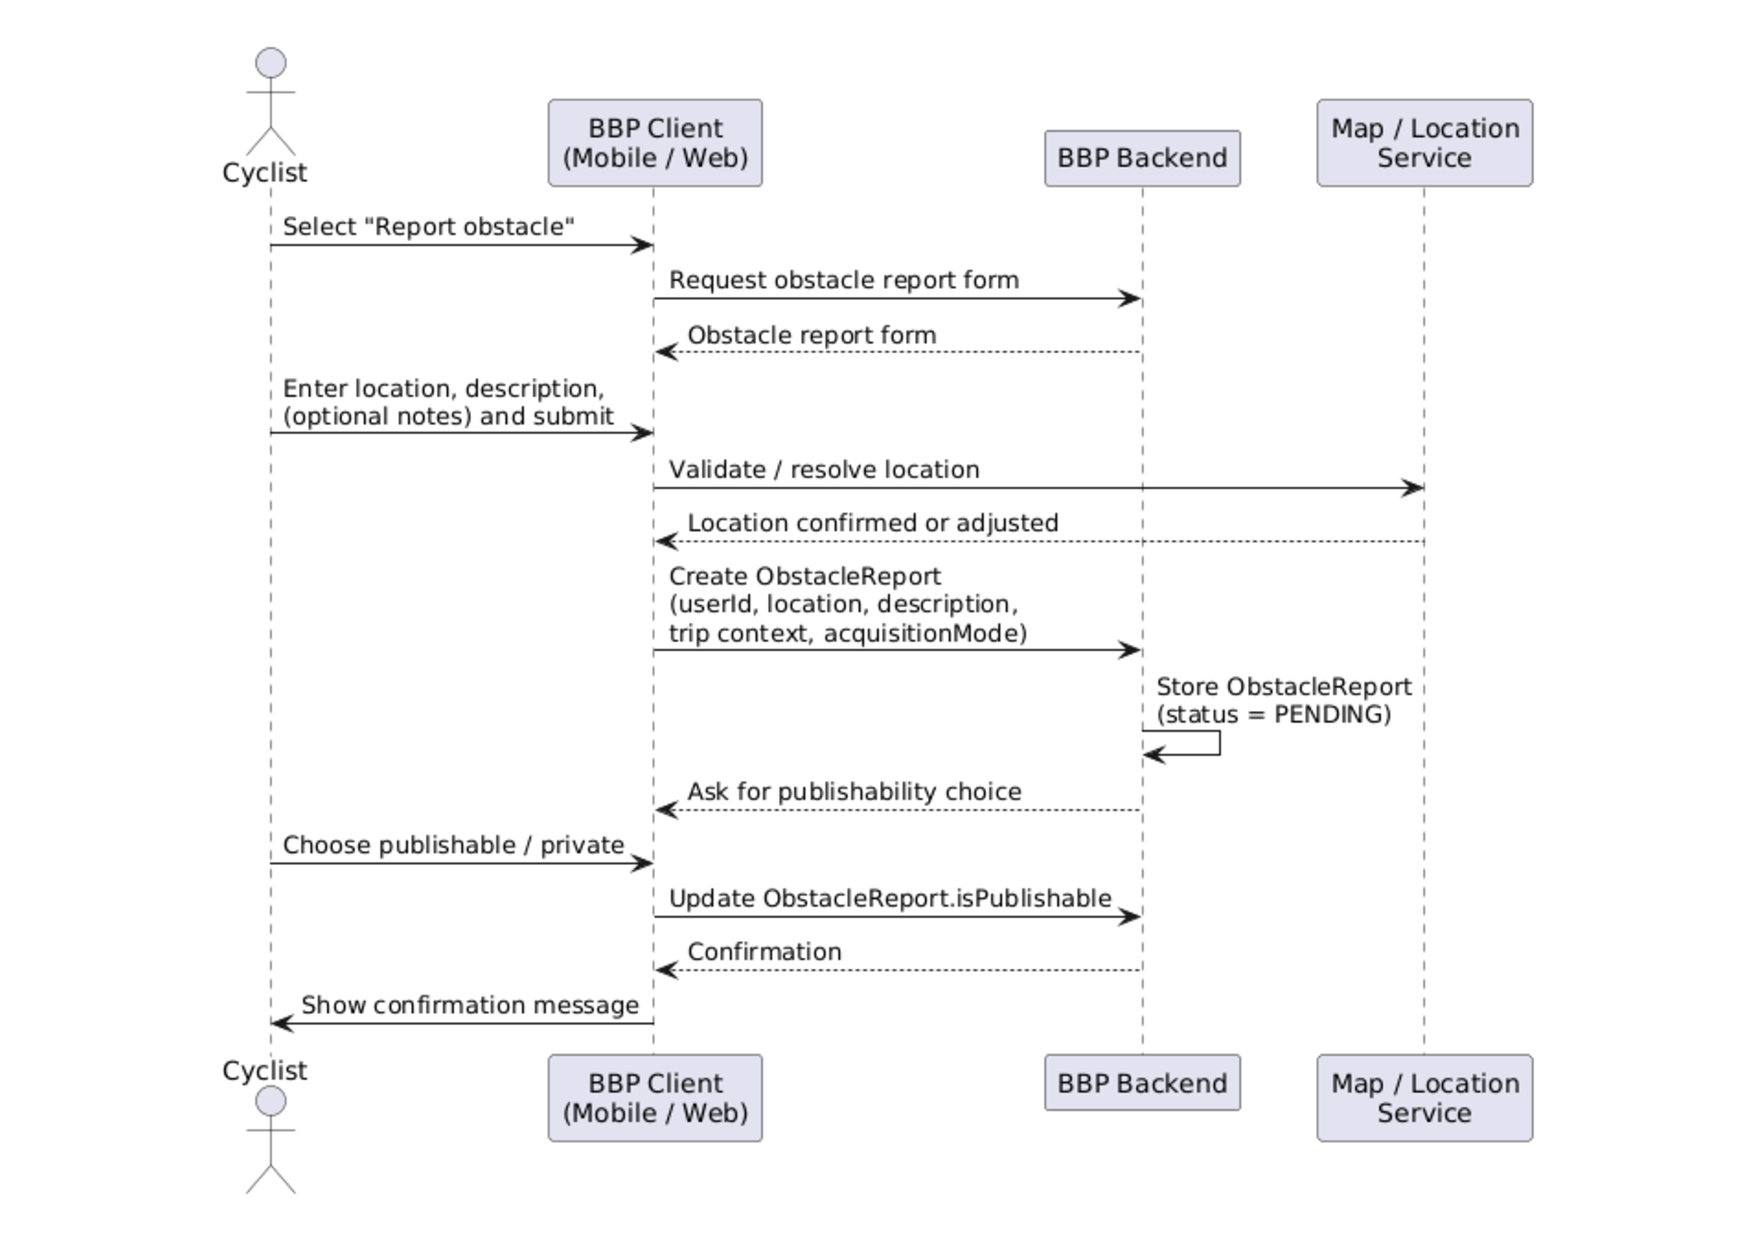
\includegraphics[width=1.0\textwidth]{Images/UC/UC_5.pdf}
    \caption{Submit obstacle report - Sequence Diagram}
    \label{fig:use-case-diagram-uc05}
\end{figure}

% ============================
% UC06: VALIDATE DETECTED OBSTACLE
% ============================

\subsubsection{UC06: Validate detected obstacle}
\label{subsubsec:validate-obstacle}

\begin{center}
\begin{longtable}{|l|p{0.75\linewidth}|}
    \hline
    \textbf{Actors:}           
    & Cyclist (registered user)                                                                      \\
    \hline

    \textbf{Entry Conditions:} 
    & \begin{itemize}
          \item The cyclist is authenticated in the BBP system.
          \item At least one \texttt{ObstacleReport} with status \texttt{PENDING} is available in the area of the cyclist or along a recorded trip.
       \end{itemize}                                                                                 \\
    \hline

    \textbf{Flow of Events:}   
    & \begin{enumerate}
          \item During or after a trip, BBP notifies the cyclist about one or more potential obstacles (pending reports) near the current path or location.
          \item The cyclist opens the obstacle notification or the obstacle list.
          \item BBP displays details of the selected pending \texttt{ObstacleReport}, including location and description.
          \item The cyclist inspects the area and chooses to either \emph{Confirm} or \emph{Reject} the obstacle.
          \item The cyclist submits their choice.
          \item BBP sends the updated decision to the backend.
          \item The backend updates the \texttt{ObstacleReport.status} to:
                \begin{itemize}
                    \item \texttt{CONFIRMED} if the cyclist confirms the obstacle;
                    \item \texttt{REJECTED} if the cyclist rejects the obstacle.
                \end{itemize}
          \item If the report is confirmed and sufficient evidence exists (for example enough confirmed reports in the same area), the backend associates the report with an existing \texttt{Obstacle} or creates a new one.
          \item BBP informs the cyclist that the obstacle report has been updated.
       \end{enumerate}                                                                                \\
    \hline

    \textbf{Exit condition:}   
    & The selected \texttt{ObstacleReport} has status \texttt{CONFIRMED} or \texttt{REJECTED}. Confirmed reports may contribute to creating or updating an \texttt{Obstacle}. \\
    \hline

    \textbf{Exceptions:}       
    & \begin{enumerate}
          \item The pending report is no longer available (for example already validated by others): BBP informs the cyclist and refreshes the list.
          \item Backend temporarily unavailable: BBP displays an error message and suggests retrying later.
          \item The cyclist closes the notification without making a choice: no change occurs to the report.
       \end{enumerate}                                                                                \\
    \hline
\end{longtable}
\end{center}

\begin{figure}[H]
    \centering
    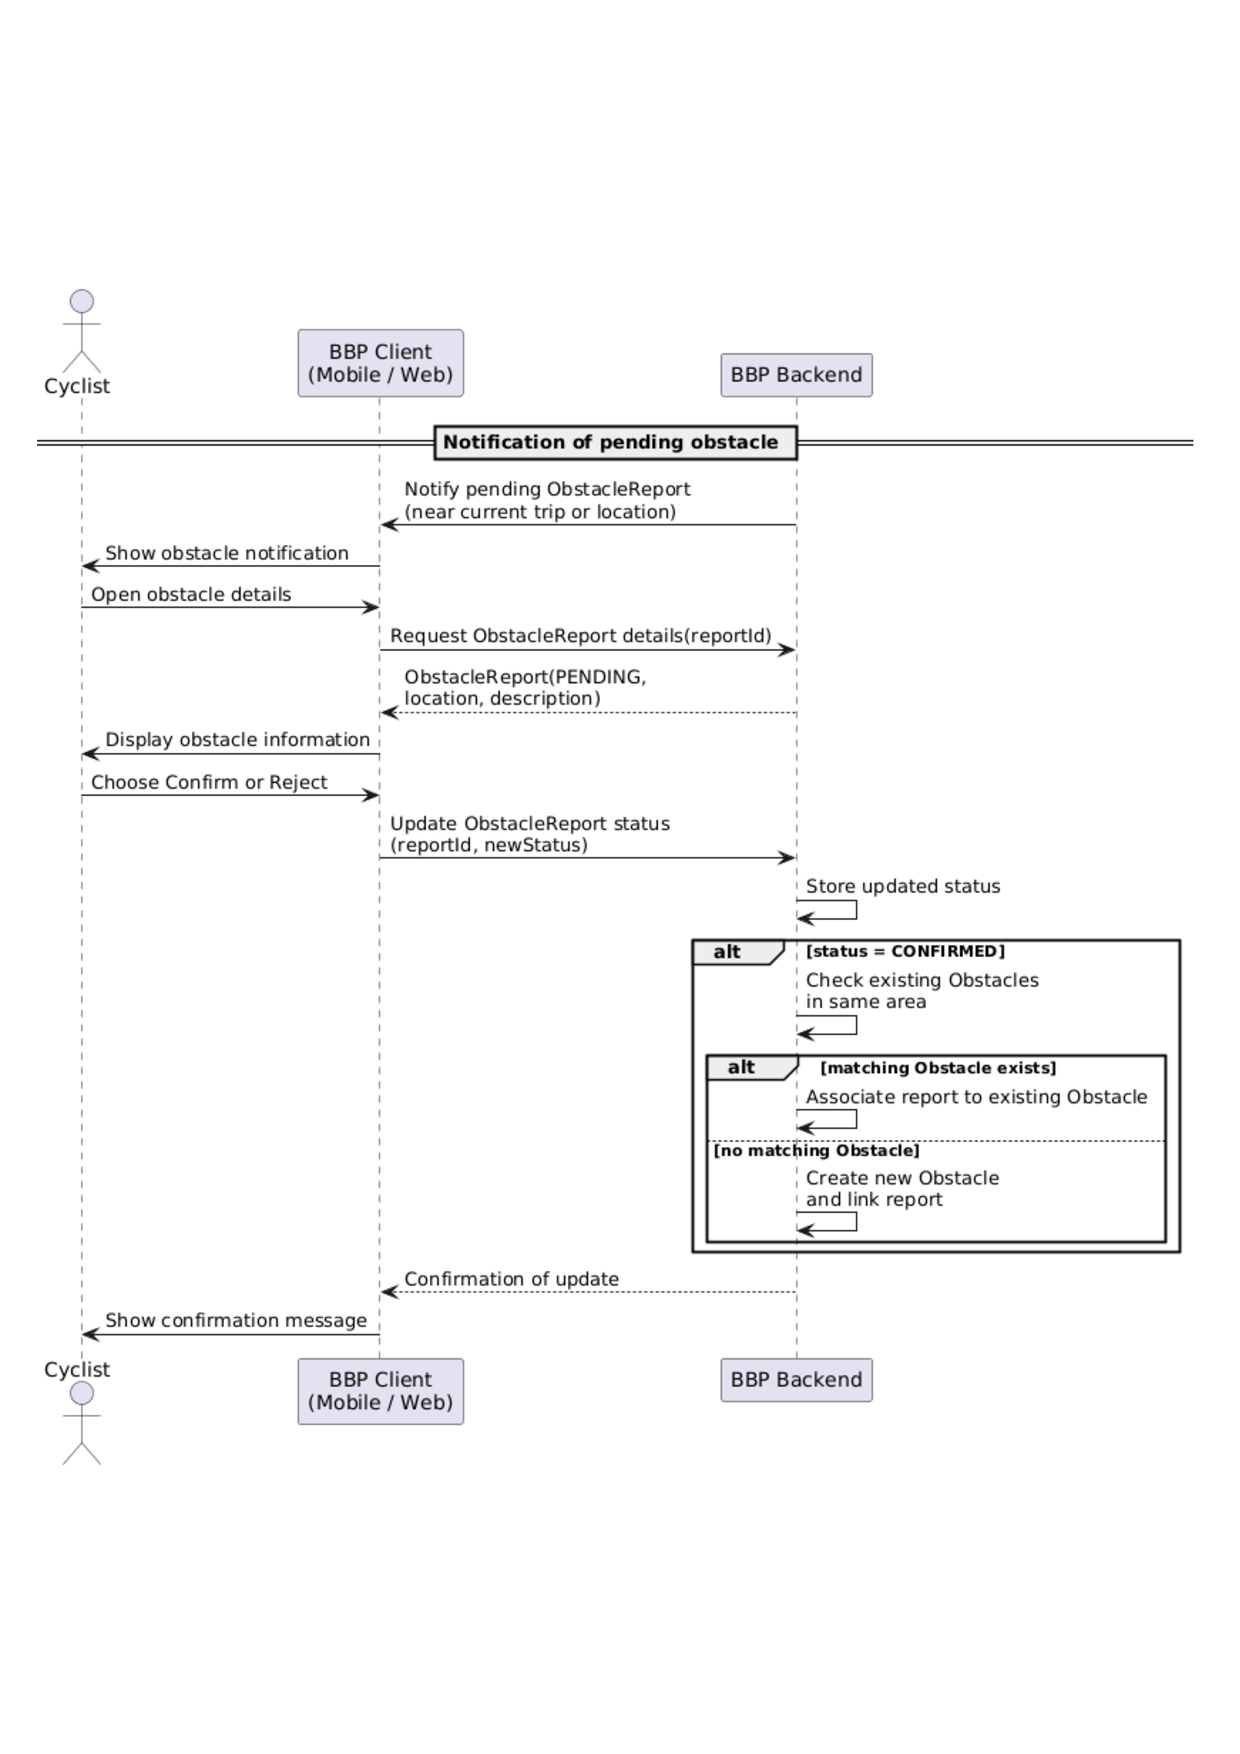
\includegraphics[width=1.0\textwidth]{Images/UC/UC_6.pdf}
    \caption{Validate detected obstacle - Use Case Diagram}
    \label{fig:use-case-diagram-uc06}
\end{figure}



\subsubsection{UC07: Browse bike paths and conditions}
\label{subsubsec:browse-bike-paths}

\begin{center}
\begin{longtable}{|l|p{0.75\linewidth}|}
    \hline
    \textbf{Actors:}           
    & Cyclist (registered or unregistered user)                                               \\
    \hline

    \textbf{Entry Conditions:} 
    & \begin{itemize}
          \item The BBP system is reachable.
          \item At least one BikePath exists in the system.
       \end{itemize}                                                                          \\
    \hline

    \textbf{Flow of Events:}   
    & \begin{enumerate}
          \item The cyclist navigates to the “Bike Paths” section of the application.
          \item BBP requests the list of BikePaths from the backend.
          \item The backend returns a list of available paths, each with:
                \begin{itemize}
                    \item origin and destination,
                    \item aggregated status,
                    \item score,
                    \item number of obstacles or reports.
                \end{itemize}
          \item The cyclist selects a specific BikePath from the list.
          \item BBP requests detailed information for the selected path.
          \item The backend returns detailed data such as:
                \begin{itemize}
                    \item its composing Streets,
                    \item existing Obstacles on those streets,
                    \item aggregated PathStatusReports.
                \end{itemize}
          \item BBP displays the complete path information to the cyclist.
       \end{enumerate}                                                                         \\
    \hline

    \textbf{Exit condition:}   
    & The cyclist visualizes detailed information of the selected BikePath.                   \\
    \hline

    \textbf{Exceptions:}       
    & \begin{enumerate}
          \item No BikePaths exist: BBP displays an empty state message.
          \item Map or backend services unavailable: BBP shows an error and suggests retrying.
          \item Some Street or Obstacle information cannot be retrieved: BBP displays partial data with a warning.
       \end{enumerate}                                                                         \\
    \hline
\end{longtable}
\end{center}

\begin{figure}[H]
    \centering
    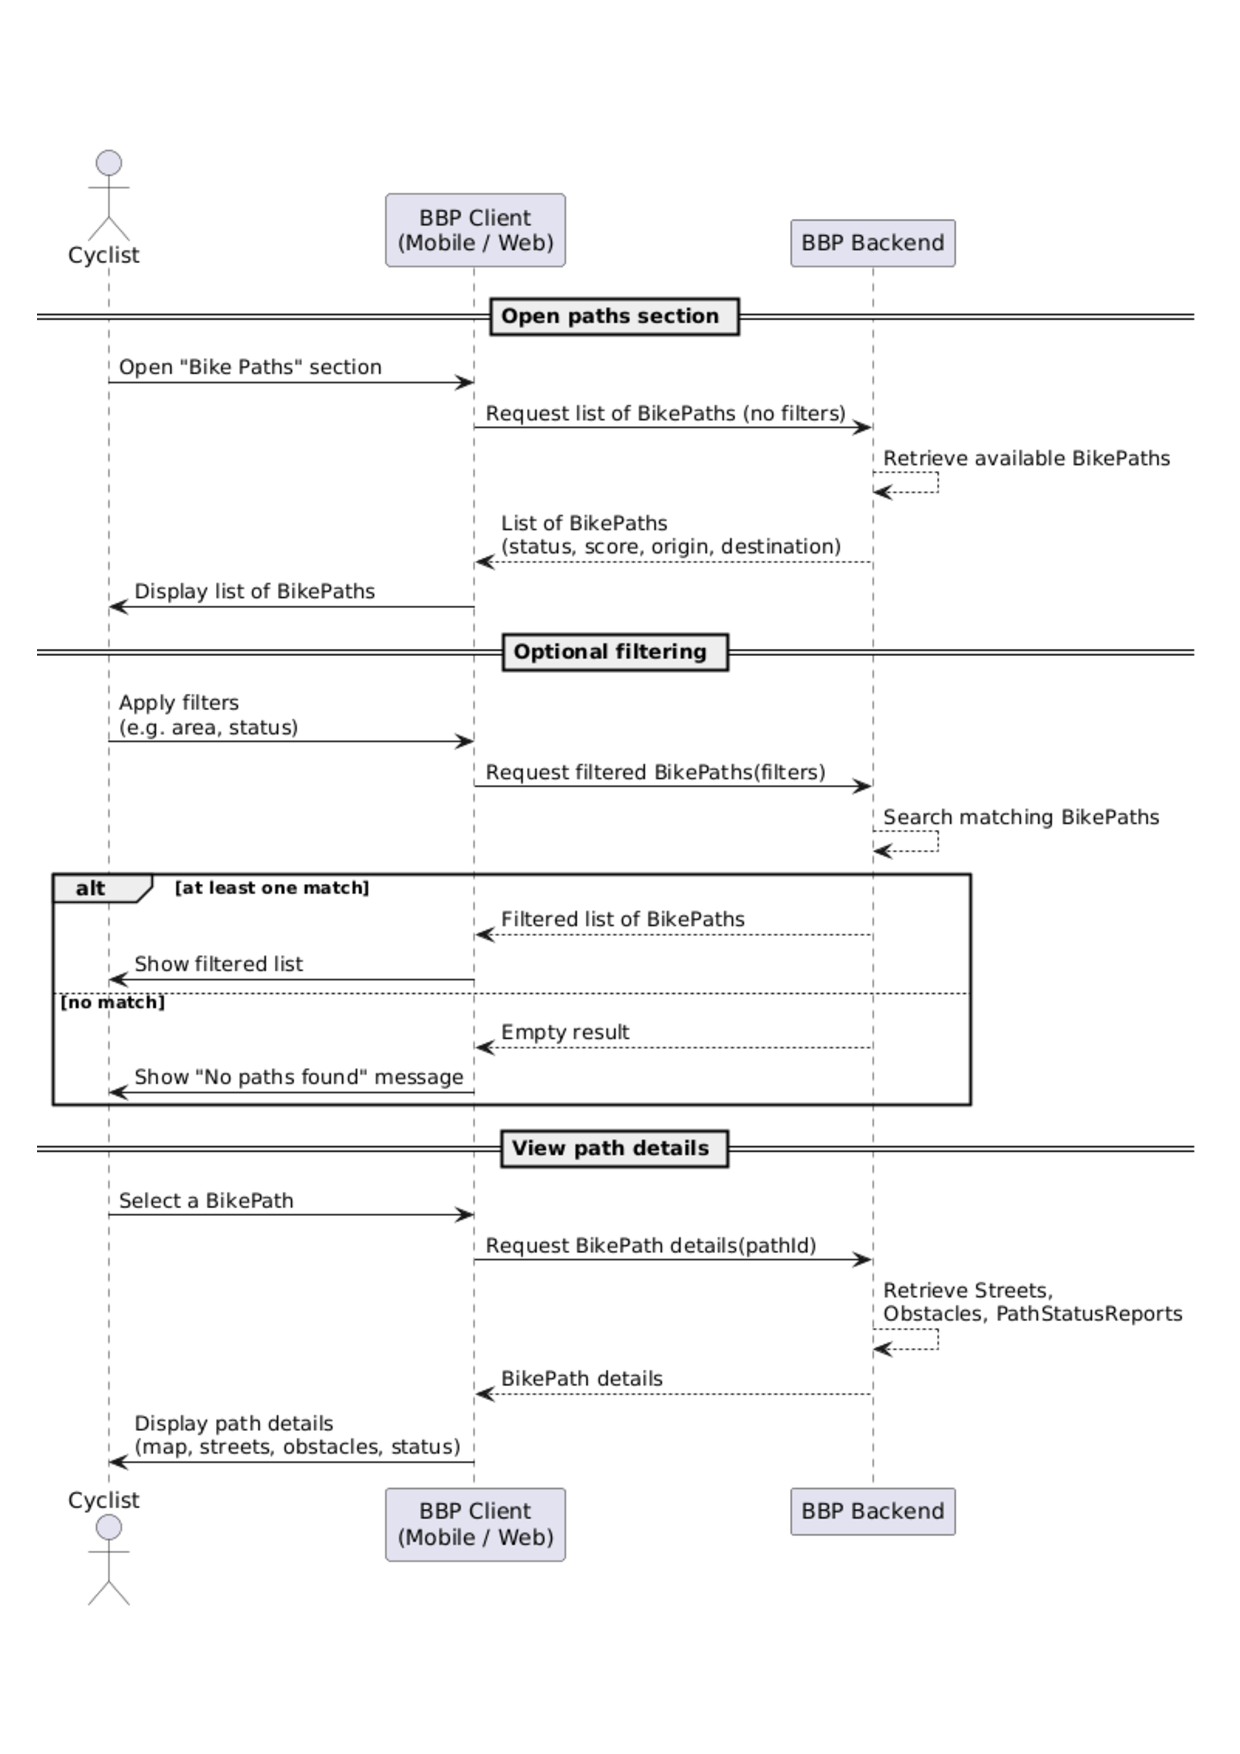
\includegraphics[width=1.0\textwidth]{Images/UC/UC_7.pdf}
    \caption{Submit obstacle report - Sequence Diagram}
    \label{fig:use-case-diagram-uc05}
\end{figure}

\subsubsection{UC08: Submit path status report}
\label{subsubsec:submit-path-status-report}

\begin{center}
\begin{longtable}{|l|p{0.75\linewidth}|}
    \hline
    \textbf{Actors:}           
    & Cyclist (registered user)                                                                 \\
    \hline

    \textbf{Entry Conditions:} 
    & \begin{itemize}
          \item The cyclist is authenticated in the BBP system.
          \item At least one \texttt{BikePath} is available in the system.
       \end{itemize}                                                                            \\
    \hline

    \textbf{Flow of Events:}   
    & \begin{enumerate}
          \item The cyclist navigates to the “Bike Paths” section and selects a specific BikePath.
          \item BBP displays detailed information of the selected path (streets, status, known obstacles).
          \item The cyclist chooses the option \emph{Rate path condition}.
          \item BBP shows a form where the cyclist can:
                \begin{itemize}
                    \item select a \texttt{PathStatus} value (e.g., OPTIMAL, MEDIUM, SUFFICIENT, REQUIRES\_MAINTENANCE);
                    \item optionally add comments;
                    \item choose whether the report should be publishable to other users.
                \end{itemize}
          \item The cyclist fills in the form and confirms the submission.
          \item BBP sends the path status report data to the backend.
          \item The backend creates a new \texttt{PathStatusReport} associated with:
                \begin{itemize}
                    \item the selected BikePath,
                    \item the current cyclist,
                    \item the selected PathStatus,
                    \item the acquisition mode (MANUAL or AUTOMATIC, if derived from a trip),
                    \item the chosen \texttt{isPublishable} setting,
                    \item the current timestamp as \texttt{createdAt}.
                \end{itemize}
          \item The backend updates the aggregated status or score of the BikePath based on the new report.
          \item BBP displays a confirmation message and the updated status (if visible to the cyclist).
       \end{enumerate}                                                                          \\
    \hline

    \textbf{Exit condition:}   
    & A new \texttt{PathStatusReport} is stored and linked to the selected BikePath and cyclist; the path’s aggregated status/score is updated. \\
    \hline

    \textbf{Exceptions:}       
    & \begin{enumerate}
          \item The cyclist does not select any status value: BBP highlights the missing field and does not submit the report.
          \item The selected BikePath no longer exists or cannot be retrieved: BBP shows an error and returns to the path list.
          \item The backend is temporarily unavailable: BBP notifies the cyclist and suggests retrying later; no report is stored.
       \end{enumerate}                                                                          \\
    \hline
\end{longtable}
\end{center}

\begin{figure}[H]
    \centering
    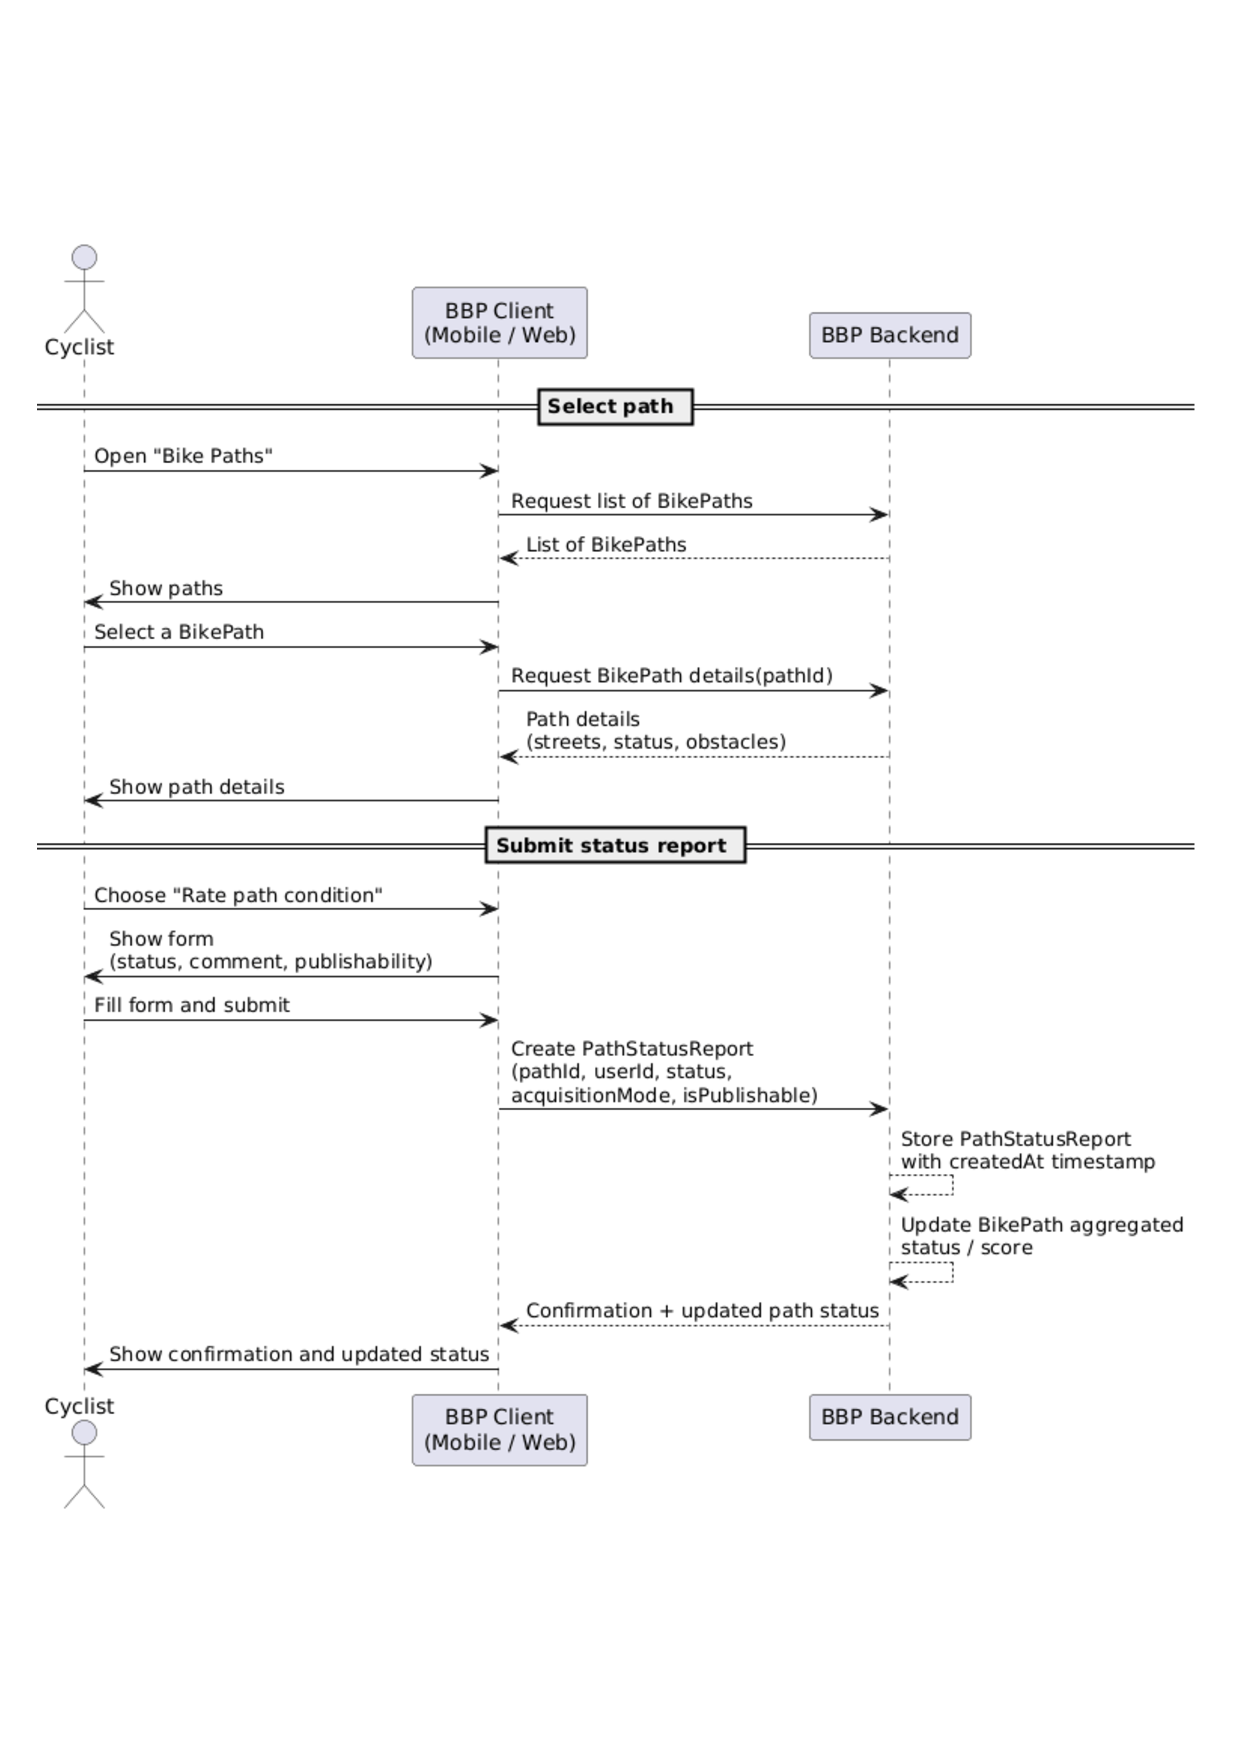
\includegraphics[width=1.0\textwidth]{Images/UC/UC_8.pdf}
    \caption{Submit obstacle report - Sequence Diagram}
    \label{fig:use-case-diagram-uc05}
\end{figure}


\subsubsection{UC09: Manage data publishability}
\label{subsubsec:manage-publishability}

\begin{center}
\begin{longtable}{|l|p{0.75\linewidth}|}
    \hline
    \textbf{Actors:}           
    & Cyclist (registered user)                                                                      \\
    \hline

    \textbf{Entry Conditions:} 
    & \begin{itemize}
          \item The cyclist is authenticated in the BBP system.
          \item The cyclist has at least one contribution stored in the system (e.g., ObstacleReport or PathStatusReport).
       \end{itemize}                                                                                 \\
    \hline

    \textbf{Flow of Events:}   
    & \begin{enumerate}
          \item The cyclist navigates to the \emph{My contributions} section of the application.
          \item BBP requests from the backend the list of contributions associated with the cyclist, including their current publishability status.
          \item The backend returns the list of contributions (e.g., obstacle reports and path status reports) with their \texttt{isPublishable} flag.
          \item BBP displays the contributions along with controls (e.g., toggles or checkboxes) for changing publishability.
          \item The cyclist changes the publishability setting for one or more contributions.
          \item The cyclist confirms the changes.
          \item BBP sends the updated publishability choices to the backend.
          \item The backend updates the \texttt{isPublishable} field for the specified contributions.
          \item BBP displays a confirmation that the publishability settings have been updated.
       \end{enumerate}                                                                                \\
    \hline

    \textbf{Exit condition:}   
    & The \texttt{isPublishable} flags of the selected contributions are updated according to the cyclist’s choices. Private items are no longer visible to other users. \\
    \hline

    \textbf{Exceptions:}       
    & \begin{enumerate}
          \item No contributions exist: BBP displays an empty state message indicating there is nothing to manage.
          \item Backend temporarily unavailable: BBP notifies the cyclist that changes could not be saved and suggests retrying later.
          \item A specific contribution cannot be updated (e.g., already deleted or invalid): BBP shows an error for that item and leaves its previous status unchanged.
       \end{enumerate}                                                                                \\
    \hline
\end{longtable}
\end{center}

\begin{figure}[H]
    \centering
    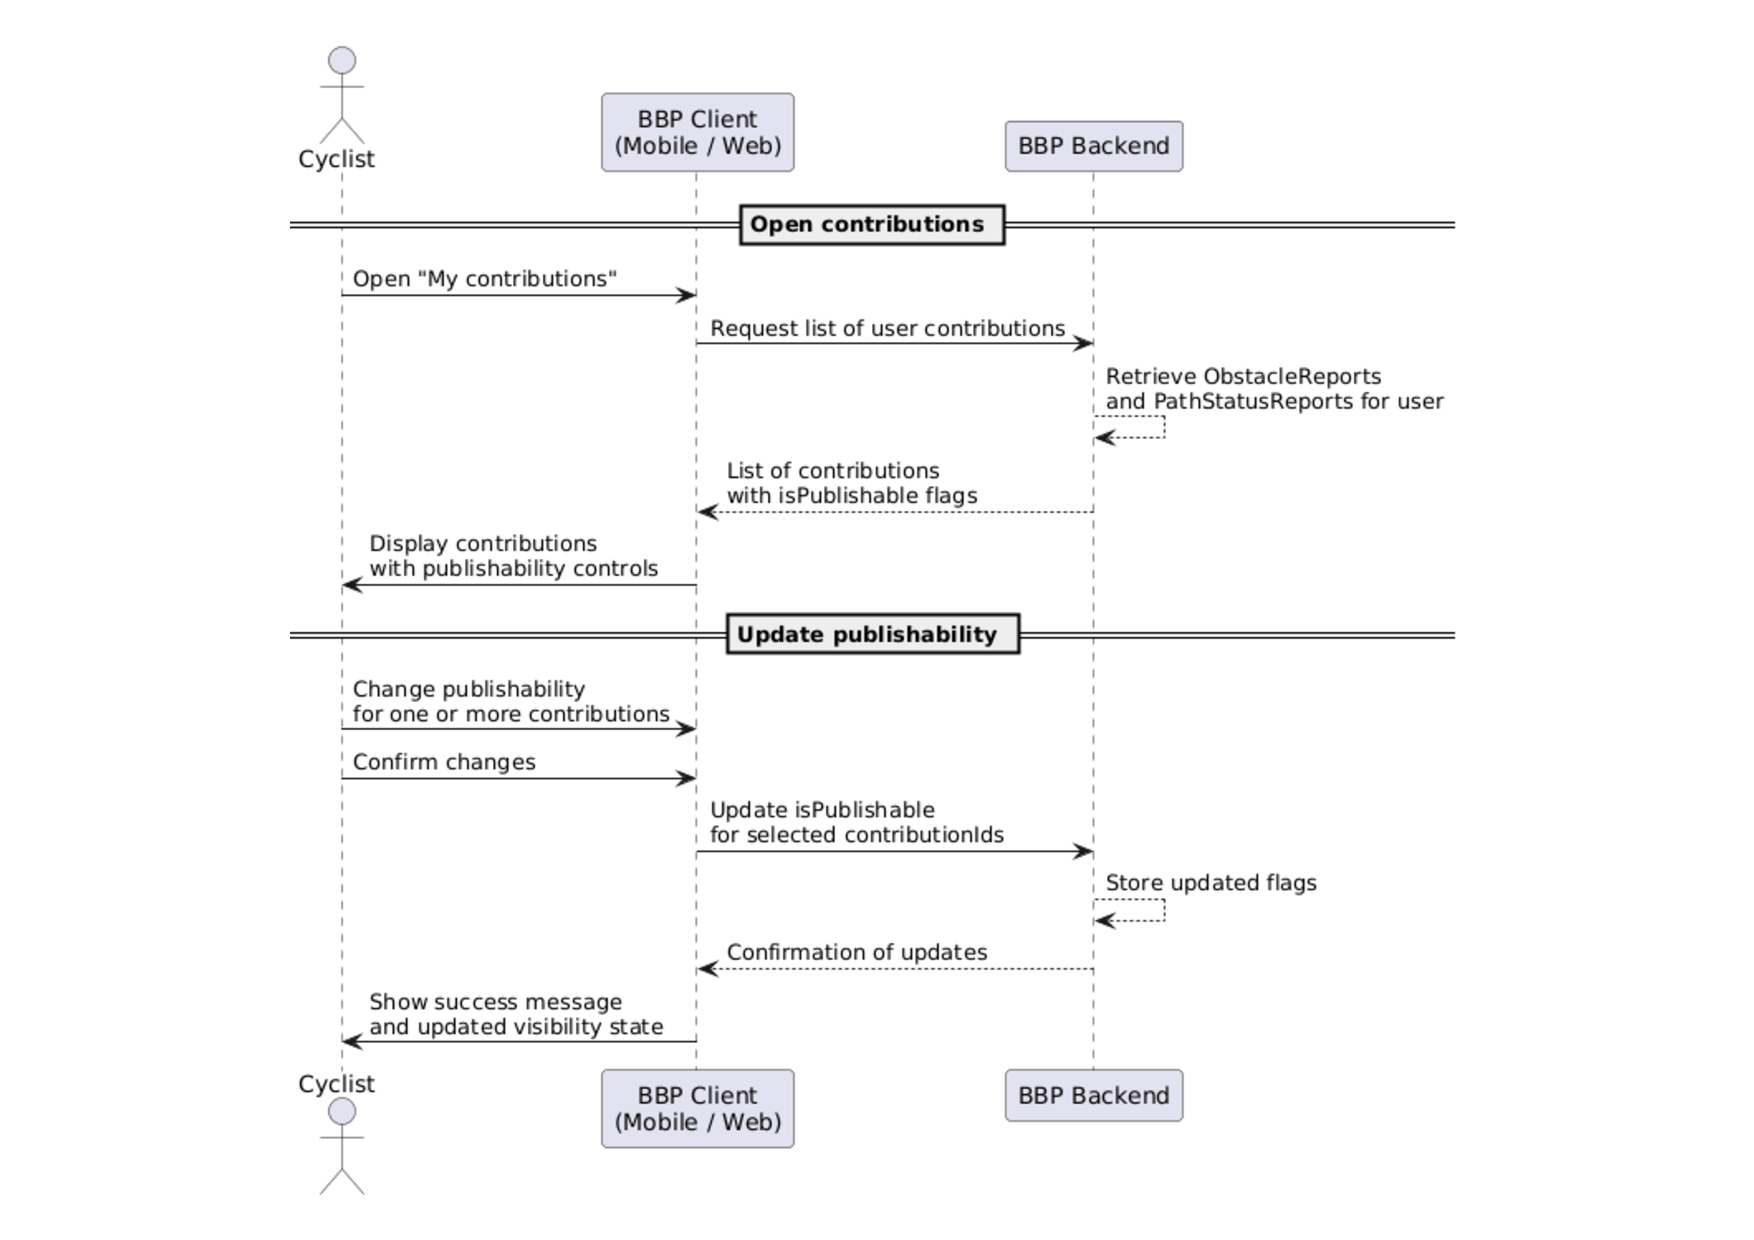
\includegraphics[width=1.0\textwidth]{Images/UC/UC_9.pdf}
    \caption{Manage data publishability - Use Case Diagram}
    \label{fig:use-case-diagram-uc09}
\end{figure}

\begin{figure}[H]
    \centering
    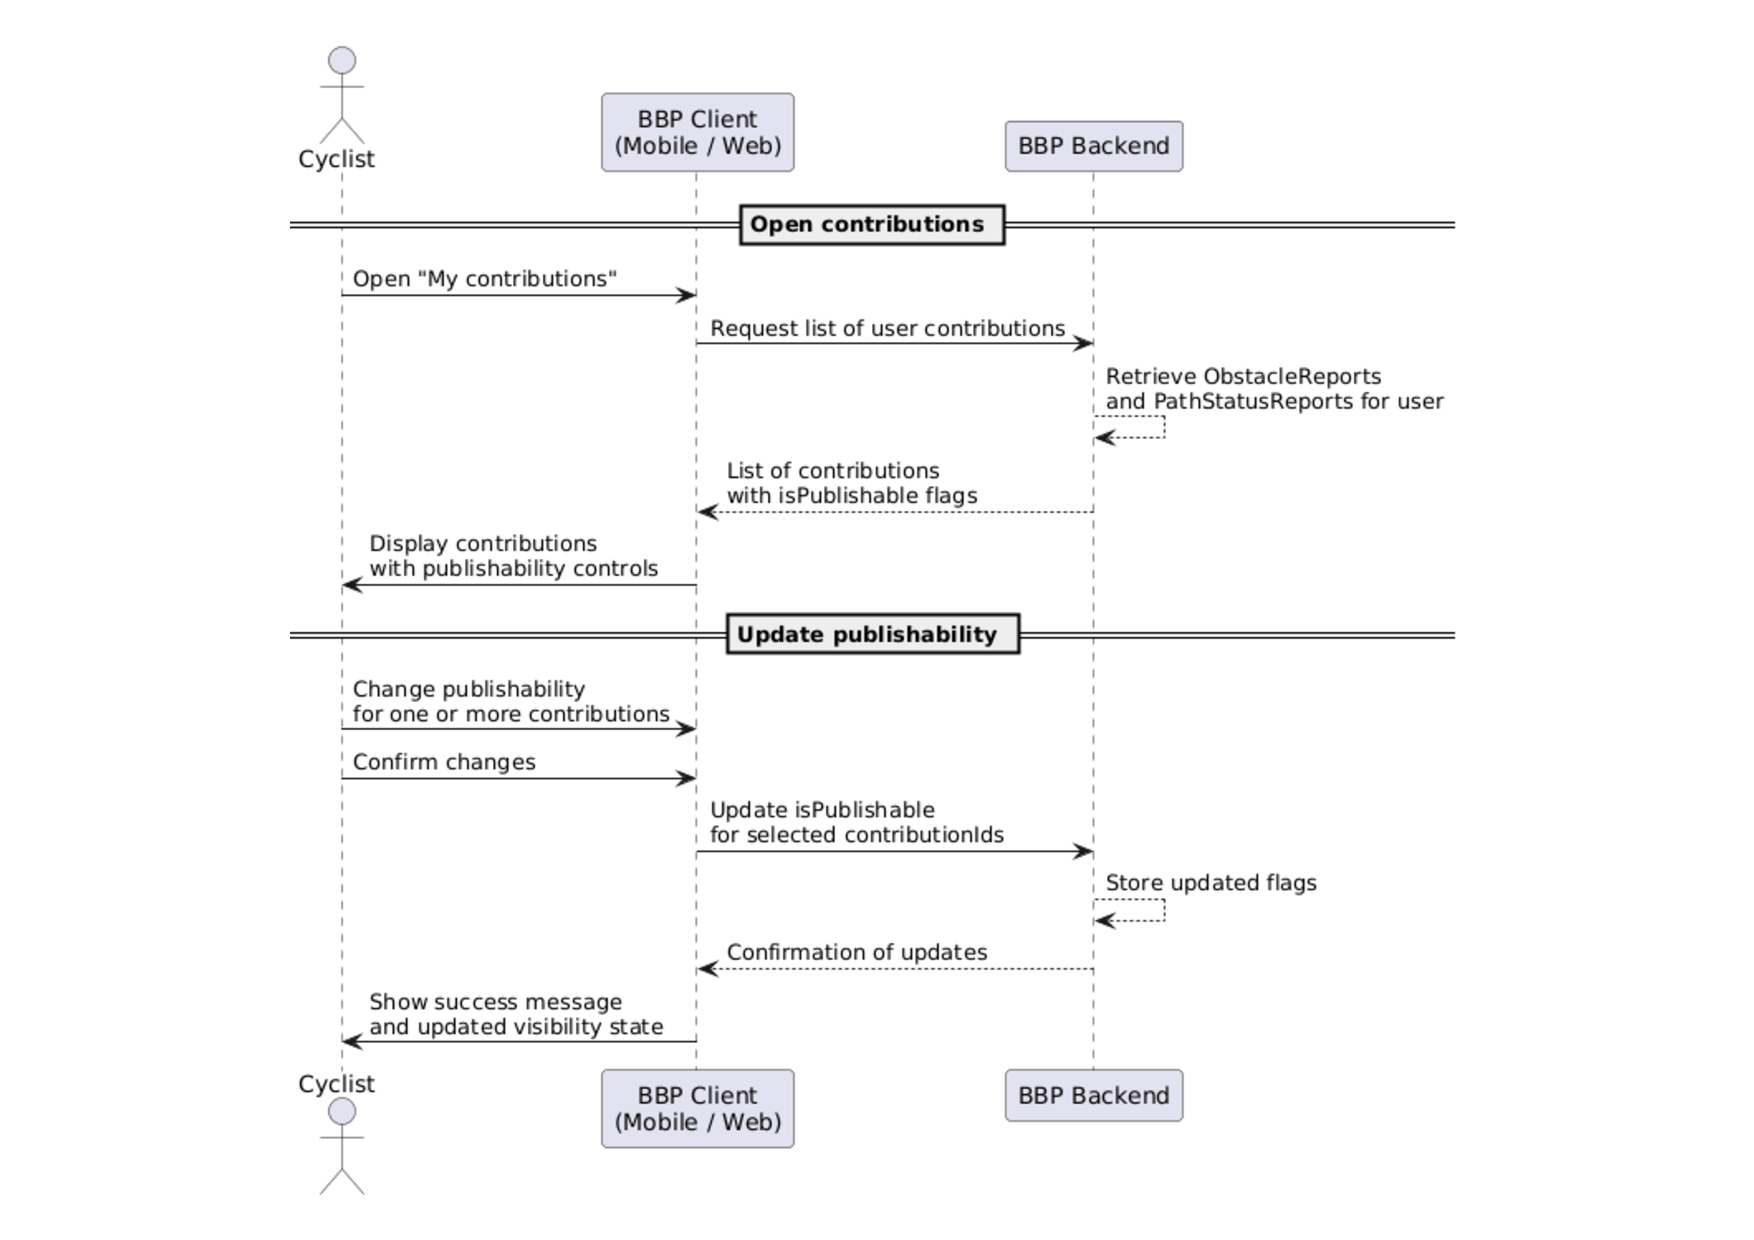
\includegraphics[width=1.0\textwidth]{Images/UC/UC_9}
    \caption{Manage data publishability - Sequence Diagram}
    \label{fig:sequence-diagram-uc09}
\end{figure}

\subsection{Goals - Requirements Mapping}
\label{subsec:goals-requirements-mapping}

\par The following table summarizes how each high-level goal of BBP is supported by one or more
functional requirements listed in Table~\ref{tab:requirements-table}. Each requirement identifier
(R01, R02, \dots, R35) refers to the corresponding entry in the Requirements List.

\begin{longtable}{|l|p{0.8\textwidth}|}
    \hline
    \textbf{Goal} & \textbf{Related Requirements} \\
    \hline \hline

    G01 & R01, R02 \\
    \hline
    \multicolumn{2}{|p{0.8\textwidth}|}{Allow the registered user (RU) to create and manage a personal account.} \\
    \hline \hline

    G02 & R04, R05, R06, R07, R08, R09, R27, R28, R33, R34 \\
    \hline
    \multicolumn{2}{|p{0.8\textwidth}|}{Allow the RU to record private personal trips (manual or automatic).} \\
    \hline \hline

    G03 & R07, R28 \\
    \hline
    \multicolumn{2}{|p{0.8\textwidth}|}{Allow the RU to view detailed statistics for each trip (distance, speed, performance metrics).} \\
    \hline \hline

    G04 & R08, R10, R20, R21, R22, R24 \\
    \hline
    \multicolumn{2}{|p{0.8\textwidth}|}{Allow the RU to manually insert path information by selecting streets and specifying their status.} \\
    \hline \hline

    G05 & R04, R05, R06, R33, R34 \\
    \hline
    \multicolumn{2}{|p{0.8\textwidth}|}{Allow the RU to collect automatic trip data via mobile sensors (GPS, accelerometer, gyroscope).} \\
    \hline \hline

    G06 & R11, R13, R14, R15, R16, R18, R19, R35 \\
    \hline
    \multicolumn{2}{|p{0.8\textwidth}|}{Allow the RU to confirm or correct automatically inferred obstacles or street conditions.} \\
    \hline \hline

    G07 & R20, R21, R22, R23, R24, R25, R29, R30 \\
    \hline
    \multicolumn{2}{|p{0.8\textwidth}|}{Allow the RU to publish, edit, or delete paths they contributed (and control their visibility).} \\
    \hline \hline

    G08 & R07, R09, R27, R28 \\
    \hline
    \multicolumn{2}{|p{0.8\textwidth}|}{Allow the RU to see a dashboard summarizing their cycling activity.} \\
    \hline \hline

    G09 & R03, R20, R21, R24, R25, R26 \\
    \hline
    \multicolumn{2}{|p{0.8\textwidth}|}{Allow users to browse all published paths and their associated conditions.} \\
    \hline \hline

    G10 & R20, R25 \\
    \hline
    \multicolumn{2}{|p{0.8\textwidth}|}{Allow users to search for paths based on origin and destination.} \\
    \hline \hline

    G11 & R20, R26, R32, R17, R18 \\
    \hline
    \multicolumn{2}{|p{0.8\textwidth}|}{Allow users to view map representations of possible routes, including streets and obstacles.} \\
    \hline \hline

    G12 & R21, R24, R25, R26 \\
    \hline
    \multicolumn{2}{|p{0.8\textwidth}|}{Allow users to sort or filter paths based on score or conditions.} \\
    \hline \hline

    G13 & R07, R21, R24 \\
    \hline
    \multicolumn{2}{|p{0.8\textwidth}|}{Enable the system to compute the score of a trip/path based on its characteristics.} \\
    \hline \hline

    G14 & R09, R31 \\
    \hline
    \multicolumn{2}{|p{0.8\textwidth}|}{Enable the system to enrich trips with meteorological information from an external weather service.} \\
    \hline \hline

    G15 & R05, R11, R13, R14, R15, R33, R34, R35 \\
    \hline
    \multicolumn{2}{|p{0.8\textwidth}|}{Enable the system to detect anomalies such as potholes using sensor data and related reports.} \\
    \hline \hline

    G16 & R20, R21, R24, R26, R28 \\
    \hline
    \multicolumn{2}{|p{0.8\textwidth}|}{Enable the system to merge similar paths contributed by multiple users, considering freshness and disagreement handling.} \\
    \hline \hline

    G17 & R20, R26, R32 \\
    \hline
    \multicolumn{2}{|p{0.8\textwidth}|}{Enable the system to provide map data through a mapping API (e.g., OpenStreetMap).} \\
    \hline

    \caption{Goals to Requirements Mapping Table}
    \label{tab:goals-requirements-mapping}
\end{longtable}

\section{Performance Requirements}
\label{sec:performance-requirements}

\par{\textbf{Latency Requirements}} Regarding performance, BBP must be developed with a scalable architecture capable of assuring its users a high Quality of Experience (QoE). In particular, the latency for real-time interactions—such as starting/stopping a trip recording or submitting an obstacle report—should be less than 300ms. Map visualization and route queries, which involve complex geospatial calculations, should load within 2 seconds under normal network conditions.

\par{\textbf{Storage Requirements}} The system must safely store geospatial data and user contributions. Unlike text-based systems, BBP deals with high-frequency sensor logs. The most storage-intensive objects will be the sequences of \texttt{TrackPoints} (GPS coordinates) for recorded trips and images associated with obstacle reports (e.g., photos of potholes). An average of 50 MB/user should be allocated to account for these data types, ensuring the scalability of the application.

\par{\textbf{Architecture Sizing}} The primary market for BBP consists of urban cyclists and commuters. Assuming a launch in a major metropolitan area with a potential user base of 50,000 active daily cyclists, the system must be designed to handle high concurrency during peak commuting hours (typically 08:00-09:00 and 17:00-18:00). The infrastructure must be dynamically scalable, capable of adjusting to accommodate usage spikes during weekends or cycling events.

\section{Design Constraints}
\label{sec:design-constraints}

\subsection{Standards Compliance}
\label{subsec:standards-compliance}

\par BBP must strictly comply with EU’s GDPR regulations, which is particularly critical given the system's collection of precise geolocation data[cite: 95]. Users must explicitly grant permissions for location tracking, and the system must allow for the anonymization or deletion of trip history upon request. Furthermore, map data integration should comply with the usage policies of the chosen external map provider (e.g., OpenStreetMap).

\subsection{Hardware Limitations}
\label{subsec:hardware-limitations}

\par \textbf{Server-side:} The backend must be able to run on standard cloud infrastructure (commodity x86 hardware) to ensure cost-effectiveness and scalability.

\par \textbf{Client-side:} Unlike typical web applications, BBP has specific hardware dependencies for its core functionality. The "Automated Mode" requires a smartphone equipped with a functioning \textbf{GPS receiver}, \textbf{accelerometer}, and \textbf{gyroscope}[cite: 95]. Consequently, the primary client interface must be a native mobile application (or a Progressive Web App with sensor access) capable of running background processes for data acquisition without draining the device battery excessively.

\pagebreak

\section{Software System Attributes}
\label{sec:software-system-attributes}%

\subsection{Reliability}
\label{subsec:reliability}%

\par The system must be designed in such a way that errors can’t propagate over the whole architecture and fault can be
easily identified and isolated. Enough replicas of data and services should be implemented to ensure the reliability of
the application.

\subsection{Availability}
\label{subsec:availability}%

\par The system must be available 99.99\% (four-nines) of the time, thus allowing 52 minutes of down-time yearly.

\par Maintenance should be carried out when the impact on the clients is negligible and must be announced in advance.

\subsection{Security}
\label{subsec:security}%

\par The system implements a comprehensive authentication and authorization framework to manage user access rights.
Authentication verifies the identity of users attempting to log in, while authorization ensures that authenticated
users possess appropriate permissions for requested actions.

\par To safeguard the system's integrity, standard security measures will be implemented, including encryption of user
credentials and personal data and protection mechanisms against database query injection vulnerabilities.

\subsection{Maintainability}
\label{subsec:maintainability}%

\par The system must be modular enough to allow future expansions with limited effort and repercussion. Enough replicas
of the system must be always up to allow maintenance without impacting on user’s traffic.

\subsection{Portability}
\label{subsec:portability}%

\par The system architecture ensures portability through a clear separation of concerns. The server-side components run on standard x86 hardware or cloud containers, making them platform-independent. The client-side functionality is split: the \textit{Dashboard} and browsing features are accessible via any standard web browser, while the \textit{Trip Tracker} requires a mobile environment to access specific hardware sensors (GPS, Accelerometer).
